% Options for packages loaded elsewhere
\PassOptionsToPackage{unicode}{hyperref}
\PassOptionsToPackage{hyphens}{url}
%
\documentclass[
]{report}
\usepackage{amsmath,amssymb}
\usepackage{lmodern}
\usepackage{iftex}
\ifPDFTeX
  \usepackage[T1]{fontenc}
  \usepackage[utf8]{inputenc}
  \usepackage{textcomp} % provide euro and other symbols
\else % if luatex or xetex
  \usepackage{unicode-math}
  \defaultfontfeatures{Scale=MatchLowercase}
  \defaultfontfeatures[\rmfamily]{Ligatures=TeX,Scale=1}
\fi
% Use upquote if available, for straight quotes in verbatim environments
\IfFileExists{upquote.sty}{\usepackage{upquote}}{}
\IfFileExists{microtype.sty}{% use microtype if available
  \usepackage[]{microtype}
  \UseMicrotypeSet[protrusion]{basicmath} % disable protrusion for tt fonts
}{}
\makeatletter
\@ifundefined{KOMAClassName}{% if non-KOMA class
  \IfFileExists{parskip.sty}{%
    \usepackage{parskip}
  }{% else
    \setlength{\parindent}{0pt}
    \setlength{\parskip}{6pt plus 2pt minus 1pt}}
}{% if KOMA class
  \KOMAoptions{parskip=half}}
\makeatother
\usepackage{xcolor}
\usepackage[left=2cm,right=2cm,top=2cm,bottom=2cm]{geometry}
\usepackage{color}
\usepackage{fancyvrb}
\newcommand{\VerbBar}{|}
\newcommand{\VERB}{\Verb[commandchars=\\\{\}]}
\DefineVerbatimEnvironment{Highlighting}{Verbatim}{commandchars=\\\{\}}
% Add ',fontsize=\small' for more characters per line
\usepackage{framed}
\definecolor{shadecolor}{RGB}{248,248,248}
\newenvironment{Shaded}{\begin{snugshade}}{\end{snugshade}}
\newcommand{\AlertTok}[1]{\textcolor[rgb]{0.94,0.16,0.16}{#1}}
\newcommand{\AnnotationTok}[1]{\textcolor[rgb]{0.56,0.35,0.01}{\textbf{\textit{#1}}}}
\newcommand{\AttributeTok}[1]{\textcolor[rgb]{0.77,0.63,0.00}{#1}}
\newcommand{\BaseNTok}[1]{\textcolor[rgb]{0.00,0.00,0.81}{#1}}
\newcommand{\BuiltInTok}[1]{#1}
\newcommand{\CharTok}[1]{\textcolor[rgb]{0.31,0.60,0.02}{#1}}
\newcommand{\CommentTok}[1]{\textcolor[rgb]{0.56,0.35,0.01}{\textit{#1}}}
\newcommand{\CommentVarTok}[1]{\textcolor[rgb]{0.56,0.35,0.01}{\textbf{\textit{#1}}}}
\newcommand{\ConstantTok}[1]{\textcolor[rgb]{0.00,0.00,0.00}{#1}}
\newcommand{\ControlFlowTok}[1]{\textcolor[rgb]{0.13,0.29,0.53}{\textbf{#1}}}
\newcommand{\DataTypeTok}[1]{\textcolor[rgb]{0.13,0.29,0.53}{#1}}
\newcommand{\DecValTok}[1]{\textcolor[rgb]{0.00,0.00,0.81}{#1}}
\newcommand{\DocumentationTok}[1]{\textcolor[rgb]{0.56,0.35,0.01}{\textbf{\textit{#1}}}}
\newcommand{\ErrorTok}[1]{\textcolor[rgb]{0.64,0.00,0.00}{\textbf{#1}}}
\newcommand{\ExtensionTok}[1]{#1}
\newcommand{\FloatTok}[1]{\textcolor[rgb]{0.00,0.00,0.81}{#1}}
\newcommand{\FunctionTok}[1]{\textcolor[rgb]{0.00,0.00,0.00}{#1}}
\newcommand{\ImportTok}[1]{#1}
\newcommand{\InformationTok}[1]{\textcolor[rgb]{0.56,0.35,0.01}{\textbf{\textit{#1}}}}
\newcommand{\KeywordTok}[1]{\textcolor[rgb]{0.13,0.29,0.53}{\textbf{#1}}}
\newcommand{\NormalTok}[1]{#1}
\newcommand{\OperatorTok}[1]{\textcolor[rgb]{0.81,0.36,0.00}{\textbf{#1}}}
\newcommand{\OtherTok}[1]{\textcolor[rgb]{0.56,0.35,0.01}{#1}}
\newcommand{\PreprocessorTok}[1]{\textcolor[rgb]{0.56,0.35,0.01}{\textit{#1}}}
\newcommand{\RegionMarkerTok}[1]{#1}
\newcommand{\SpecialCharTok}[1]{\textcolor[rgb]{0.00,0.00,0.00}{#1}}
\newcommand{\SpecialStringTok}[1]{\textcolor[rgb]{0.31,0.60,0.02}{#1}}
\newcommand{\StringTok}[1]{\textcolor[rgb]{0.31,0.60,0.02}{#1}}
\newcommand{\VariableTok}[1]{\textcolor[rgb]{0.00,0.00,0.00}{#1}}
\newcommand{\VerbatimStringTok}[1]{\textcolor[rgb]{0.31,0.60,0.02}{#1}}
\newcommand{\WarningTok}[1]{\textcolor[rgb]{0.56,0.35,0.01}{\textbf{\textit{#1}}}}
\usepackage{longtable,booktabs,array}
\usepackage{calc} % for calculating minipage widths
% Correct order of tables after \paragraph or \subparagraph
\usepackage{etoolbox}
\makeatletter
\patchcmd\longtable{\par}{\if@noskipsec\mbox{}\fi\par}{}{}
\makeatother
% Allow footnotes in longtable head/foot
\IfFileExists{footnotehyper.sty}{\usepackage{footnotehyper}}{\usepackage{footnote}}
\makesavenoteenv{longtable}
\usepackage{graphicx}
\makeatletter
\def\maxwidth{\ifdim\Gin@nat@width>\linewidth\linewidth\else\Gin@nat@width\fi}
\def\maxheight{\ifdim\Gin@nat@height>\textheight\textheight\else\Gin@nat@height\fi}
\makeatother
% Scale images if necessary, so that they will not overflow the page
% margins by default, and it is still possible to overwrite the defaults
% using explicit options in \includegraphics[width, height, ...]{}
\setkeys{Gin}{width=\maxwidth,height=\maxheight,keepaspectratio}
% Set default figure placement to htbp
\makeatletter
\def\fps@figure{htbp}
\makeatother
\setlength{\emergencystretch}{3em} % prevent overfull lines
\providecommand{\tightlist}{%
  \setlength{\itemsep}{0pt}\setlength{\parskip}{0pt}}
\setcounter{secnumdepth}{5}
\ifLuaTeX
  \usepackage{selnolig}  % disable illegal ligatures
\fi
\IfFileExists{bookmark.sty}{\usepackage{bookmark}}{\usepackage{hyperref}}
\IfFileExists{xurl.sty}{\usepackage{xurl}}{} % add URL line breaks if available
\urlstyle{same} % disable monospaced font for URLs
\hypersetup{
  pdftitle={Credit card transactions fraud detection},
  pdfauthor={Edyta Pietrucha \& Anna Wieczorek},
  hidelinks,
  pdfcreator={LaTeX via pandoc}}

\title{Credit card transactions fraud detection}
\author{Edyta Pietrucha \& Anna Wieczorek}
\date{24.01.2022}

\begin{document}
\maketitle

\tableofcontents

\hypertarget{introduction}{%
\chapter{Introduction}\label{introduction}}

The project will be run with R and we will be using the following
libraries:

\begin{Shaded}
\begin{Highlighting}[]
\NormalTok{main\_path }\OtherTok{\textless{}{-}} \FunctionTok{dirname}\NormalTok{(rstudioapi}\SpecialCharTok{::}\FunctionTok{getActiveDocumentContext}\NormalTok{()}\SpecialCharTok{$}\NormalTok{path)}
\FunctionTok{setwd}\NormalTok{(main\_path)}
\FunctionTok{library}\NormalTok{(ggplot2)}
\FunctionTok{library}\NormalTok{(data.table)}
\FunctionTok{library}\NormalTok{(dplyr)}
\FunctionTok{library}\NormalTok{(tidyr)}
\FunctionTok{library}\NormalTok{(tidyverse)}
\FunctionTok{library}\NormalTok{(modelr)}
\FunctionTok{library}\NormalTok{(klaR)}
\FunctionTok{library}\NormalTok{(GGally)}
\FunctionTok{library}\NormalTok{(randomForest)}
\FunctionTok{library}\NormalTok{(gridExtra)}
\end{Highlighting}
\end{Shaded}

First, let us explain, what a credit card fraud is. We will call
unauthorized credit card transactions as \textbf{frauds}. It is a
serious problem, especially in the modern era, due to very easy to
perform internet transactions. Although banks introduced two-step
verification for shopping online, there are still people, who will find
new ways to use someone's money.

In the project we will focus on finding a model, that suites the fraud
detection best and it will be done with respect to two metrics - recall
and precision.

$$ recall = \frac{TP}{TP+FN}$$
$$ precision = \frac{TP}{TP+FP}$$

We will try to maximize recall, but also try to keep precision on a
reasonable level.

\hypertarget{data-description}{%
\chapter{Data description}\label{data-description}}

Data input:

\begin{Shaded}
\begin{Highlighting}[]
\NormalTok{data\_train }\OtherTok{\textless{}{-}} \FunctionTok{fread}\NormalTok{(}\FunctionTok{paste0}\NormalTok{(main\_path, }\StringTok{"/Data/fraudTrain.csv"}\NormalTok{))}
\NormalTok{data\_test }\OtherTok{\textless{}{-}} \FunctionTok{fread}\NormalTok{(}\FunctionTok{paste0}\NormalTok{(main\_path, }\StringTok{"Data/fraudTest.csv"}\NormalTok{))}
\end{Highlighting}
\end{Shaded}

The aim of this paper is to predict whether a transaction is fraudulent
or not. Database which we will use is a simulated credit card
transaction dataset containing legitimate and fraud transactions from
the duration 1st Jan 2019 - 31st Dec 2020. This was generated using
Sparkov Data Generation tool.

Database is available on kaggle (see the link below):

\url{https://www.kaggle.com/kartik2112/fraud-detection/version/1?select=fraudTrain.csv}

Dataset has 1296675 observations and 23 columns.

Columns of the dataset:

\begin{itemize}
\tightlist
\item
  index - Unique Identifier for each row
\item
  transdatetrans\_time - Transaction DateTime
\item
  cc\_num - Credit Card Number of Customer
\item
  merchant - Merchant Name
\item
  category - Category of Merchant
\item
  amt - Amount of Transaction
\item
  first - First Name of Credit Card Holder
\item
  last - Last Name of Credit Card Holder
\item
  gender - Gender of Credit Card Holder
\item
  street - Street Address of Credit Card Holder
\item
  city - City of Credit Card Holder
\item
  state - State of Credit Card Holder
\item
  zip - Zip of Credit Card Holder
\item
  lat - Latitude Location of Credit Card Holder
\item
  long - Longitude Location of Credit Card Holder
\item
  city\_pop - Credit Card Holder's City Population
\item
  job - Job of Credit Card Holder
\item
  dob - Date of Birth of Credit Card Holder
\item
  trans\_num - Transaction Number
\item
  unix\_time - UNIX Time of transaction
\item
  merch\_lat - Latitude Location of Merchant
\item
  merch\_long - Longitude Location of Merchant
\item
  is\_fraud - Fraud Flag (1 - fraudulent transaction, 0 - non-fraudulent
  transaction)
\end{itemize}

We will predict the chances of a fraudulent transaction in function of
the other variables.

Dataset contains 973 different holders and 983 different credit card
numbers which means that there are Customers who have more than one
credit card. We notice that each transaction number is unique.

Frequency of fraudulent transactions is approximately 0.5788652 \%. The
dataset has 0 missing values.

We notice that:

\begin{itemize}
\tightlist
\item
  X - id of observation, not helpful at all,
\item
  first, last - name of each Holder will be individual and not helpful
  as such,
\item
  street, zip - we have a location parameters so we do not use this
  variables,
\item
  unix\_time - we have transaction time which gives the same
  information,
\item
  trans\_num - is individual for each transaction and not helpful as
  such.
\end{itemize}

Therefore, we will remove those columns.

\begin{Shaded}
\begin{Highlighting}[]
\NormalTok{data\_train }\OtherTok{\textless{}{-}}\NormalTok{ data\_train }\SpecialCharTok{\%\textgreater{}\%}
\NormalTok{  .[,}\SpecialCharTok{{-}}\FunctionTok{c}\NormalTok{(}\StringTok{"V1"}\NormalTok{, }\StringTok{"first"}\NormalTok{, }\StringTok{"last"}\NormalTok{, }\StringTok{"street"}\NormalTok{, }\StringTok{"zip"}\NormalTok{, }\StringTok{"unix\_time"}\NormalTok{, }\StringTok{"trans\_num"}\NormalTok{)] }
\end{Highlighting}
\end{Shaded}

\hypertarget{data-wrangling}{%
\chapter{Data Wrangling}\label{data-wrangling}}

First, we will look at the structure of our data, to check if the
datatypes are correct.

\begin{Shaded}
\begin{Highlighting}[]
\NormalTok{data\_train }\SpecialCharTok{\%\textgreater{}\%}
\NormalTok{  str}
\end{Highlighting}
\end{Shaded}

\begin{verbatim}
## Classes 'data.table' and 'data.frame':   1296675 obs. of  16 variables:
##  $ trans_date_trans_time: POSIXct, format: "2019-01-01 00:00:18" "2019-01-01 00:00:44" ...
##  $ cc_num               :integer64 2703186189652095 630423337322 38859492057661 3534093764340240 375534208663984 4767265376804500 30074693890476 6011360759745864 ... 
##  $ merchant             : chr  "fraud_Rippin, Kub and Mann" "fraud_Heller, Gutmann and Zieme" "fraud_Lind-Buckridge" "fraud_Kutch, Hermiston and Farrell" ...
##  $ category             : chr  "misc_net" "grocery_pos" "entertainment" "gas_transport" ...
##  $ amt                  : num  4.97 107.23 220.11 45 41.96 ...
##  $ gender               : chr  "F" "F" "M" "M" ...
##  $ city                 : chr  "Moravian Falls" "Orient" "Malad City" "Boulder" ...
##  $ state                : chr  "NC" "WA" "ID" "MT" ...
##  $ lat                  : num  36.1 48.9 42.2 46.2 38.4 ...
##  $ long                 : num  -81.2 -118.2 -112.3 -112.1 -79.5 ...
##  $ city_pop             : int  3495 149 4154 1939 99 2158 2691 6018 1472 151785 ...
##  $ job                  : chr  "Psychologist, counselling" "Special educational needs teacher" "Nature conservation officer" "Patent attorney" ...
##  $ dob                  : IDate, format: "1988-03-09" "1978-06-21" ...
##  $ merch_lat            : num  36 49.2 43.2 47 38.7 ...
##  $ merch_long           : num  -82 -118.2 -112.2 -112.6 -78.6 ...
##  $ is_fraud             : int  0 0 0 0 0 0 0 0 0 0 ...
##  - attr(*, ".internal.selfref")=<externalptr>
\end{verbatim}

We can see, that we will need to convert some variables to factors.

\begin{Shaded}
\begin{Highlighting}[]
\NormalTok{dt }\OtherTok{\textless{}{-}} \FunctionTok{c}\NormalTok{(}\StringTok{"cc\_num"}\NormalTok{, }\StringTok{"merchant"}\NormalTok{, }\StringTok{"category"}\NormalTok{, }\StringTok{"gender"}\NormalTok{, }\StringTok{"city"}\NormalTok{, }\StringTok{"state"}\NormalTok{, }\StringTok{"job"}\NormalTok{, }\StringTok{"is\_fraud"}\NormalTok{)}
\NormalTok{data\_train[,(dt)}\SpecialCharTok{:}\ErrorTok{=} \FunctionTok{lapply}\NormalTok{(.SD, as.factor), .SDcols }\OtherTok{=}\NormalTok{ dt]}
\end{Highlighting}
\end{Shaded}

We need to convert \texttt{trans\_date\_trans\_time} and \texttt{dob} to
date class for further analysis.

\begin{Shaded}
\begin{Highlighting}[]
\NormalTok{data\_train[, dob }\SpecialCharTok{:}\ErrorTok{=} \FunctionTok{as.Date}\NormalTok{(dob)]}
\NormalTok{data\_train[, trans\_date\_trans\_time }\SpecialCharTok{:}\ErrorTok{=} \FunctionTok{strptime}\NormalTok{(trans\_date\_trans\_time,}
                                               \AttributeTok{format =}\StringTok{"\%Y{-}\%m{-}\%d \%H:\%M:\%OS"}\NormalTok{, }
                                               \AttributeTok{tz =} \StringTok{"EST"}\NormalTok{)]}
\end{Highlighting}
\end{Shaded}

Now, let us look at the data structure again:

\begin{Shaded}
\begin{Highlighting}[]
\NormalTok{data\_train }\SpecialCharTok{\%\textgreater{}\%}
\NormalTok{  str}
\end{Highlighting}
\end{Shaded}

\begin{verbatim}
## Classes 'data.table' and 'data.frame':   1296675 obs. of  16 variables:
##  $ trans_date_trans_time: POSIXct, format: "2019-01-01 00:00:18" "2019-01-01 00:00:44" ...
##  $ cc_num               : Factor w/ 983 levels "60416207185",..: 445 43 238 510 369 755 158 821 777 454 ...
##  $ merchant             : Factor w/ 693 levels "fraud_Abbott-Rogahn",..: 516 244 390 364 298 608 534 108 251 565 ...
##  $ category             : Factor w/ 14 levels "entertainment",..: 9 5 1 3 10 3 4 3 10 5 ...
##  $ amt                  : num  4.97 107.23 220.11 45 41.96 ...
##  $ gender               : Factor w/ 2 levels "F","M": 1 1 2 2 2 1 1 2 1 1 ...
##  $ city                 : Factor w/ 894 levels "Achille","Acworth",..: 527 613 469 85 217 224 352 237 475 150 ...
##  $ state                : Factor w/ 51 levels "AK","AL","AR",..: 28 48 14 27 46 39 17 46 39 43 ...
##  $ lat                  : num  36.1 48.9 42.2 46.2 38.4 ...
##  $ long                 : num  -81.2 -118.2 -112.3 -112.1 -79.5 ...
##  $ city_pop             : int  3495 149 4154 1939 99 2158 2691 6018 1472 151785 ...
##  $ job                  : Factor w/ 494 levels "Academic librarian",..: 371 429 308 329 117 480 30 128 376 330 ...
##  $ dob                  : Date, format: "1988-03-09" "1978-06-21" ...
##  $ merch_lat            : num  36 49.2 43.2 47 38.7 ...
##  $ merch_long           : num  -82 -118.2 -112.2 -112.6 -78.6 ...
##  $ is_fraud             : Factor w/ 2 levels "0","1": 1 1 1 1 1 1 1 1 1 1 ...
##  - attr(*, ".internal.selfref")=<externalptr>
\end{verbatim}

And the types are correct now.

\hypertarget{explanatory-data-analysis}{%
\section{Explanatory Data Analysis}\label{explanatory-data-analysis}}

All functions used in project can be found in the Appendix.

\hypertarget{age}{%
\subsection{Age}\label{age}}

We created a new variable which counts age of each Customer in a day of
a transaction. We assume that age of a Holder can have an impact on
detecting fraudulent transactions, especially combined with variables
such as amount of money spent on a transaction or transacion time.

\begin{Shaded}
\begin{Highlighting}[]
\NormalTok{data\_train[, age }\SpecialCharTok{:}\ErrorTok{=} \FunctionTok{round}\NormalTok{(}\FunctionTok{as.numeric}\NormalTok{(}\FunctionTok{difftime}\NormalTok{(trans\_date\_trans\_time, dob, }\AttributeTok{units =} \StringTok{"days"}\NormalTok{)}\SpecialCharTok{/}\DecValTok{365}\NormalTok{), }\DecValTok{0}\NormalTok{)]}
\end{Highlighting}
\end{Shaded}

Data visualization:

\begin{Shaded}
\begin{Highlighting}[]
\FunctionTok{ggplot}\NormalTok{(data\_train, }\FunctionTok{aes}\NormalTok{(}\AttributeTok{x =}\NormalTok{ is\_fraud, }\AttributeTok{y =}\NormalTok{ age)) }\SpecialCharTok{+}
  \FunctionTok{geom\_boxplot}\NormalTok{() }\SpecialCharTok{+}
\NormalTok{  my\_style }\SpecialCharTok{+}
  \FunctionTok{labs}\NormalTok{(}\AttributeTok{title =} \StringTok{"Boxplot for age of Customer"}\NormalTok{,}
       \AttributeTok{subtitle=}\StringTok{"group by not{-}fraudulent transactions and fraudulent transactions"}\NormalTok{)}
\end{Highlighting}
\end{Shaded}

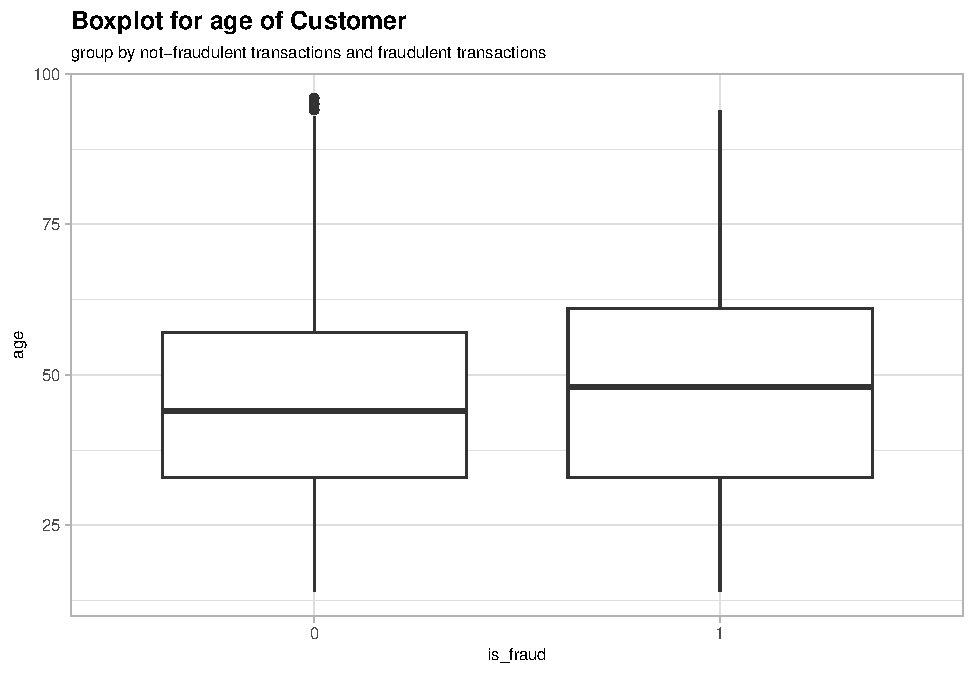
\includegraphics{credit_card_fraud_detection_files/figure-latex/age_plot-1.pdf}
Mean for fraudulent transactions is a little bit higher than for
not-fraudulent transactions.

\hypertarget{gender}{%
\subsection{Gender}\label{gender}}

Further analysis has led us to this conclusion that even though there
are less men than women in our data, the number of frauds for men is
slightly higher than for women.

\begin{Shaded}
\begin{Highlighting}[]
\CommentTok{\# checking a percentage of fraud transaction of each gender}
\NormalTok{gender\_fraud }\OtherTok{\textless{}{-}}\NormalTok{ data\_train }\SpecialCharTok{\%\textgreater{}\%} 
\NormalTok{  .[, .(}\AttributeTok{count =}\NormalTok{ .N), by }\OtherTok{=} \FunctionTok{c}\NormalTok{(}\StringTok{"gender"}\NormalTok{, }\StringTok{"is\_fraud"}\NormalTok{)] }\SpecialCharTok{\%\textgreater{}\%}
\NormalTok{  .[, .(is\_fraud, }\AttributeTok{freq =}\NormalTok{ count}\SpecialCharTok{/}\FunctionTok{sum}\NormalTok{(count)), by }\OtherTok{=}\NormalTok{ gender] }\SpecialCharTok{\%\textgreater{}\%}
\NormalTok{  .[is\_fraud }\SpecialCharTok{==} \DecValTok{1}\NormalTok{]}
\NormalTok{gender\_fraud}
\end{Highlighting}
\end{Shaded}

\begin{verbatim}
##    gender is_fraud        freq
## 1:      F        1 0.005261579
## 2:      M        1 0.006426249
\end{verbatim}

Visualize the data:

\begin{Shaded}
\begin{Highlighting}[]
\FunctionTok{ggplot}\NormalTok{(gender\_fraud, }\FunctionTok{aes}\NormalTok{(}\AttributeTok{x =}\NormalTok{ gender, }\AttributeTok{y =}\NormalTok{ freq, }\AttributeTok{fill =}\NormalTok{ gender)) }\SpecialCharTok{+}
  \FunctionTok{geom\_bar}\NormalTok{(}\AttributeTok{stat =} \StringTok{\textquotesingle{}identity\textquotesingle{}}\NormalTok{) }\SpecialCharTok{+}
\NormalTok{  my\_style }\SpecialCharTok{+}
  \FunctionTok{scale\_fill\_manual}\NormalTok{(}\AttributeTok{values =} \FunctionTok{c}\NormalTok{(my\_palette[}\FunctionTok{c}\NormalTok{(}\DecValTok{4}\NormalTok{,}\DecValTok{7}\NormalTok{)])) }\SpecialCharTok{+}
  \FunctionTok{labs}\NormalTok{(}\AttributeTok{title =} \StringTok{"Frequency of fraud group by gender"}\NormalTok{,}
       \AttributeTok{x =} \StringTok{""}\NormalTok{,}
       \AttributeTok{y =} \StringTok{""}\NormalTok{)}
\end{Highlighting}
\end{Shaded}

\begin{figure}
\centering
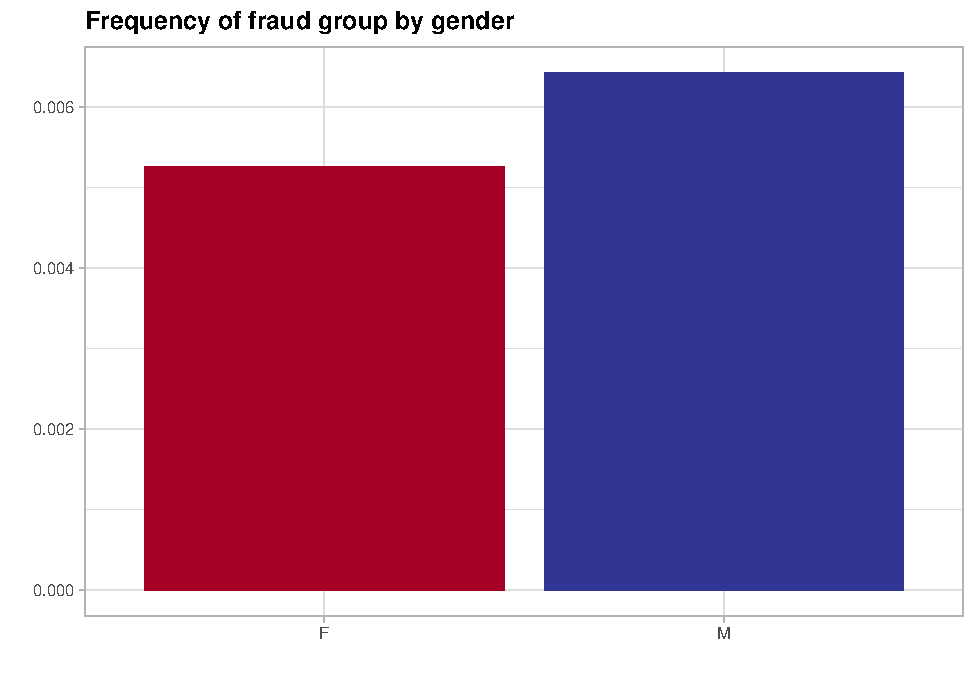
\includegraphics{credit_card_fraud_detection_files/figure-latex/gender_plot -1.pdf}
\caption{\label{Fig:gender_plot}Frequency of fraudulent transactions
group by gender.}
\end{figure}

\hypertarget{amt}{%
\subsection{Amt}\label{amt}}

Variable \texttt{amt} corresponds to the amount of money spent on each
transaction. We assume that this information can have a huge impact to
detect if a transaction is fraudulent. Let's see basic statistics for
\texttt{amt}.

Mean and median amount of fraudulent transactions are higher than for
not-fraudulent transactions.

We would like to create a boxplot to visualize datapoints, but we
detected to much outliers in observations for not-fraudlent
transactions. To deal with that problem we created our own function
which removes outliers from a dataset.

\begin{Shaded}
\begin{Highlighting}[]
\NormalTok{remove\_outlier }\OtherTok{\textless{}{-}} \ControlFlowTok{function}\NormalTok{(data, column) \{}
  
\NormalTok{  IQR }\OtherTok{\textless{}{-}} \FunctionTok{quantile}\NormalTok{(data[, }\FunctionTok{get}\NormalTok{(column)], }\FloatTok{0.75}\NormalTok{) }\SpecialCharTok{{-}} \FunctionTok{quantile}\NormalTok{(data[, }\FunctionTok{get}\NormalTok{(column)], }\FloatTok{0.25}\NormalTok{) }\CommentTok{\# IQR= Q3 (75\% quantile) – Q1 (25\% quantile)}
  \CommentTok{\# Outlier would be a point below [Q1{-} (1.5)IQR] or above [Q3+(1.5)IQR]}
\NormalTok{  l }\OtherTok{\textless{}{-}} \FunctionTok{quantile}\NormalTok{(data[, }\FunctionTok{get}\NormalTok{(column)], }\FloatTok{0.25}\NormalTok{) }\SpecialCharTok{{-}} \FloatTok{1.5}\SpecialCharTok{*}\NormalTok{IQR}
\NormalTok{  r }\OtherTok{\textless{}{-}} \FunctionTok{quantile}\NormalTok{(data[, }\FunctionTok{get}\NormalTok{(column)], }\FloatTok{0.75}\NormalTok{) }\SpecialCharTok{+} \FloatTok{1.5}\SpecialCharTok{*}\NormalTok{IQR}
  
\NormalTok{  data }\OtherTok{\textless{}{-}}\NormalTok{ data }\SpecialCharTok{\%\textgreater{}\%}
\NormalTok{    .[}\FunctionTok{get}\NormalTok{(column) }\SpecialCharTok{\textgreater{}=}\NormalTok{ l }\SpecialCharTok{\&} \FunctionTok{get}\NormalTok{(column) }\SpecialCharTok{\textless{}=}\NormalTok{ r]}
  
  \FunctionTok{return}\NormalTok{(data)}
  
\NormalTok{\}}
\end{Highlighting}
\end{Shaded}

\begin{Shaded}
\begin{Highlighting}[]
\FunctionTok{ggplot}\NormalTok{(}\FunctionTok{remove\_outlier}\NormalTok{(data\_train, }\StringTok{"amt"}\NormalTok{), }
       \FunctionTok{aes}\NormalTok{(}\AttributeTok{x =}\NormalTok{ is\_fraud, }\AttributeTok{y =}\NormalTok{ amt)) }\SpecialCharTok{+}
  \FunctionTok{geom\_boxplot}\NormalTok{() }\SpecialCharTok{+}
\NormalTok{  my\_style }\SpecialCharTok{+}
  \FunctionTok{labs}\NormalTok{(}\AttributeTok{title =} \StringTok{"Boxplot for amount spent on the transaction"}\NormalTok{,}
       \AttributeTok{subtitle =} \StringTok{"group by not{-}fraudulent transactions and fraudulent transactions"}\NormalTok{)}
\end{Highlighting}
\end{Shaded}

\begin{figure}
\centering
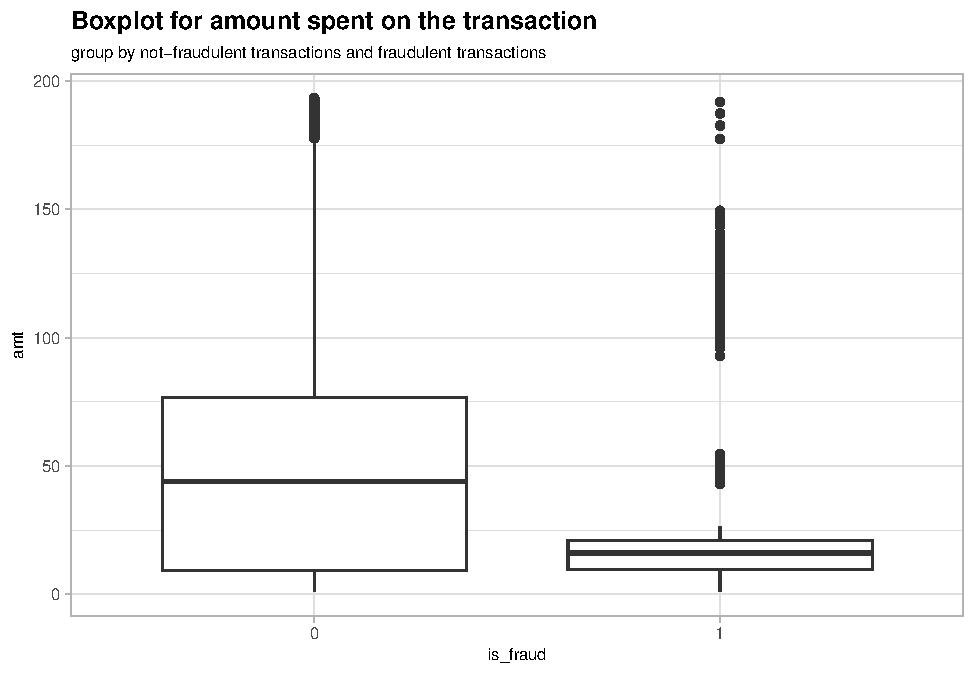
\includegraphics{credit_card_fraud_detection_files/figure-latex/amt_plot-1.pdf}
\caption{\label{Fig:amt_plot}Boxplot for variable amt group by
not-fraudulent transactions and fraudulent transactions.}
\end{figure}

Graphic analysis confirms our assumptions that the variable \texttt{amt}
can be really important for aim of our project.

\hypertarget{weekday-of-transaction}{%
\subsection{Weekday of transaction}\label{weekday-of-transaction}}

We think, that the weekday of a transaction could be an important
indicator of fraudulent transactions, especially when combined with
other variables like the amount of money spent on purchase or the
transaction hour. So we decided to create a variable
\texttt{week\_day\_trans} to conduct the analysis.

\begin{Shaded}
\begin{Highlighting}[]
\NormalTok{data\_train[, week\_day\_of\_trans }\SpecialCharTok{:}\ErrorTok{=} \FunctionTok{as.factor}\NormalTok{(}\FunctionTok{wday}\NormalTok{(trans\_date\_trans\_time))]}
\end{Highlighting}
\end{Shaded}

\begin{Shaded}
\begin{Highlighting}[]
\NormalTok{week\_day\_fraud }\OtherTok{\textless{}{-}}\NormalTok{ data\_train }\SpecialCharTok{\%\textgreater{}\%} 
\NormalTok{  .[, .(}\AttributeTok{count =}\NormalTok{ .N), by }\OtherTok{=} \FunctionTok{c}\NormalTok{(}\StringTok{"week\_day\_of\_trans"}\NormalTok{, }\StringTok{"is\_fraud"}\NormalTok{)] }\SpecialCharTok{\%\textgreater{}\%}
\NormalTok{  .[, .(is\_fraud, }\AttributeTok{freq =}\NormalTok{ count}\SpecialCharTok{/}\FunctionTok{sum}\NormalTok{(count)), by }\OtherTok{=}\NormalTok{ week\_day\_of\_trans] }\SpecialCharTok{\%\textgreater{}\%}
\NormalTok{  .[is\_fraud }\SpecialCharTok{==} \DecValTok{1}\NormalTok{]}
\end{Highlighting}
\end{Shaded}

Once we have created the variable, we can look at the frequency of
frauds on each day. On Mondays and Tuesdays the odds of a fraudulent
transactions are slightly lower than on the other days.

\begin{Shaded}
\begin{Highlighting}[]
\FunctionTok{ggplot}\NormalTok{(week\_day\_fraud, }\FunctionTok{aes}\NormalTok{(}\AttributeTok{x =}\NormalTok{ week\_day\_of\_trans, }\AttributeTok{y =}\NormalTok{ freq, }\AttributeTok{fill =}\NormalTok{ week\_day\_of\_trans)) }\SpecialCharTok{+}
  \FunctionTok{geom\_bar}\NormalTok{(}\AttributeTok{stat =} \StringTok{\textquotesingle{}identity\textquotesingle{}}\NormalTok{) }\SpecialCharTok{+}
\NormalTok{  my\_style }\SpecialCharTok{+}
  \FunctionTok{scale\_fill\_manual}\NormalTok{(}\AttributeTok{values =} \FunctionTok{c}\NormalTok{(my\_palette[}\DecValTok{1}\SpecialCharTok{:}\DecValTok{7}\NormalTok{])) }\SpecialCharTok{+}
  \FunctionTok{labs}\NormalTok{(}\AttributeTok{title =} \StringTok{"Frequency of fraud group by weekday of the transaction"}\NormalTok{,}
       \AttributeTok{x =} \StringTok{""}\NormalTok{,}
       \AttributeTok{y =} \StringTok{""}\NormalTok{) }\SpecialCharTok{+}
  \FunctionTok{scale\_x\_discrete}\NormalTok{(}\AttributeTok{labels=}\FunctionTok{c}\NormalTok{(}\StringTok{"Monday"}\NormalTok{, }\StringTok{"Tuesday"}\NormalTok{, }\StringTok{"Wednesday"}\NormalTok{, }\StringTok{"Thursday"}\NormalTok{,}
                            \StringTok{"Friday"}\NormalTok{, }\StringTok{"Saturday"}\NormalTok{, }\StringTok{"Sunday"}\NormalTok{))}
\end{Highlighting}
\end{Shaded}

\begin{figure}
\centering
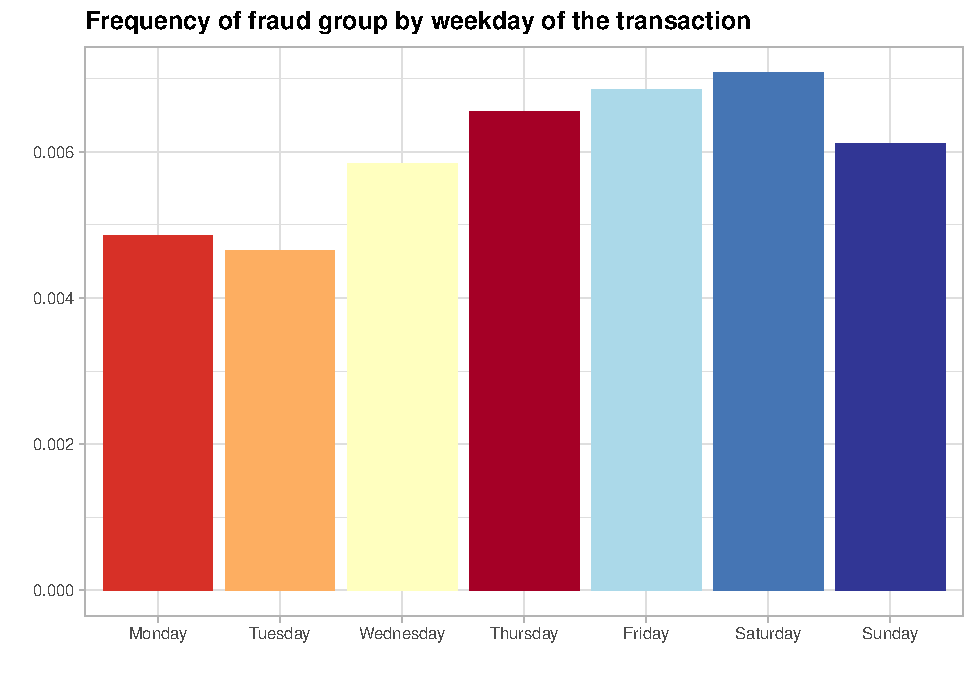
\includegraphics{credit_card_fraud_detection_files/figure-latex/weekday_plot-1.pdf}
\caption{\label{Fig:weekday_plot}Frequancy of fraudulent transactions
grouped by the weekday.}
\end{figure}

\hypertarget{category-of-purchase}{%
\subsection{Category of Purchase}\label{category-of-purchase}}

Investigating the data, we see that some categories, that is:
\emph{grocery\_pos}, \emph{misc\_net}, \emph{shopping\_net} and
\emph{shopping\_pos}, seem to be more vulnerable to fraudulent
transactions than others.

\begin{Shaded}
\begin{Highlighting}[]
\NormalTok{category\_fraud }\OtherTok{\textless{}{-}}\NormalTok{ data\_train }\SpecialCharTok{\%\textgreater{}\%} 
\NormalTok{  .[, .(}\AttributeTok{count =}\NormalTok{ .N), by }\OtherTok{=} \FunctionTok{c}\NormalTok{(}\StringTok{"category"}\NormalTok{, }\StringTok{"is\_fraud"}\NormalTok{)] }\SpecialCharTok{\%\textgreater{}\%}
\NormalTok{  .[, .(is\_fraud, }\AttributeTok{freq =}\NormalTok{ count}\SpecialCharTok{/}\FunctionTok{sum}\NormalTok{(count)), by }\OtherTok{=}\NormalTok{ category] }\SpecialCharTok{\%\textgreater{}\%}
\NormalTok{  .[is\_fraud }\SpecialCharTok{==} \DecValTok{1}\NormalTok{]}
\end{Highlighting}
\end{Shaded}

\begin{Shaded}
\begin{Highlighting}[]
\FunctionTok{ggplot}\NormalTok{(category\_fraud, }\FunctionTok{aes}\NormalTok{(}\AttributeTok{x =}\NormalTok{ category, }\AttributeTok{y =}\NormalTok{ freq, }\AttributeTok{fill =}\NormalTok{ category)) }\SpecialCharTok{+}
  \FunctionTok{geom\_bar}\NormalTok{(}\AttributeTok{stat =} \StringTok{\textquotesingle{}identity\textquotesingle{}}\NormalTok{) }\SpecialCharTok{+}
\NormalTok{  my\_style }\SpecialCharTok{+}
  \FunctionTok{labs}\NormalTok{(}\AttributeTok{title =} \StringTok{"Frequency of fraud group by category of merchant"}\NormalTok{,}
       \AttributeTok{x =} \StringTok{""}\NormalTok{,}
       \AttributeTok{y =} \StringTok{""}\NormalTok{) }\SpecialCharTok{+}
  \FunctionTok{coord\_flip}\NormalTok{()}
\end{Highlighting}
\end{Shaded}

\begin{figure}
\centering
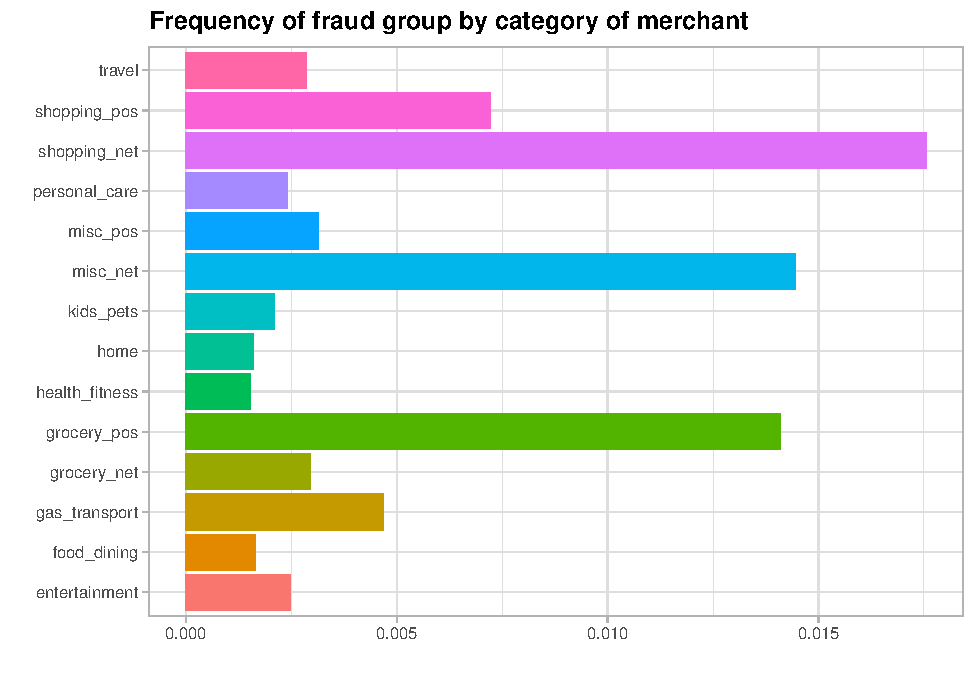
\includegraphics{credit_card_fraud_detection_files/figure-latex/category_plot-1.pdf}
\caption{\label{Fig:category_plot}Frequancy of fraudulent transactions
grouped by the category of purchase.}
\end{figure}

We can see this phenomenon on the Figure \ref{Fig:category_plot}.

\hypertarget{transaction-date-transaction-time}{%
\subsection{Transaction date, transaction
time}\label{transaction-date-transaction-time}}

Let us dive into transaction date and time in more details. First, we
will create a variable \texttt{trans\_hour} and see if at any time of
the day, such as late night, chance of fraud is higher.

\begin{Shaded}
\begin{Highlighting}[]
\NormalTok{data\_train[, trans\_hour }\SpecialCharTok{:}\ErrorTok{=} \FunctionTok{as\_factor}\NormalTok{(}\FunctionTok{strftime}\NormalTok{(trans\_date\_trans\_time, }
                                              \AttributeTok{format=}\StringTok{"\%H"}\NormalTok{, }
                                              \AttributeTok{tz =} \StringTok{"EST"}\NormalTok{))]}
\end{Highlighting}
\end{Shaded}

\begin{Shaded}
\begin{Highlighting}[]
\NormalTok{hour\_fraud }\OtherTok{\textless{}{-}}\NormalTok{ data\_train }\SpecialCharTok{\%\textgreater{}\%}
\NormalTok{  .[, .(}\AttributeTok{count =}\NormalTok{ .N), by }\OtherTok{=} \FunctionTok{c}\NormalTok{(}\StringTok{"trans\_hour"}\NormalTok{, }\StringTok{"is\_fraud"}\NormalTok{)] }\SpecialCharTok{\%\textgreater{}\%}
\NormalTok{  .[, .(is\_fraud, }\AttributeTok{freq =}\NormalTok{ count}\SpecialCharTok{/}\FunctionTok{sum}\NormalTok{(count)), by }\OtherTok{=}\NormalTok{ trans\_hour] }\SpecialCharTok{\%\textgreater{}\%}
\NormalTok{  .[is\_fraud }\SpecialCharTok{==} \DecValTok{1}\NormalTok{]}
\end{Highlighting}
\end{Shaded}

As expected, at night the frequency of frauds is much higher than during
a day. This insight, combined with the age of a Holder can be very
important for our model. For example, it is much more likely that a
younger person will be buying something at night, than an elderly one.

\begin{Shaded}
\begin{Highlighting}[]
\FunctionTok{ggplot}\NormalTok{(hour\_fraud, }\FunctionTok{aes}\NormalTok{(}\AttributeTok{x =}\NormalTok{ trans\_hour, }\AttributeTok{y =}\NormalTok{ freq, }\AttributeTok{fill =}\NormalTok{ trans\_hour)) }\SpecialCharTok{+}
  \FunctionTok{geom\_bar}\NormalTok{(}\AttributeTok{stat =} \StringTok{\textquotesingle{}identity\textquotesingle{}}\NormalTok{) }\SpecialCharTok{+}
\NormalTok{  my\_style }\SpecialCharTok{+}
  \FunctionTok{labs}\NormalTok{(}\AttributeTok{title =} \StringTok{"Frequency of fraud group by transaction hour"}\NormalTok{,}
       \AttributeTok{x =} \StringTok{""}\NormalTok{,}
       \AttributeTok{y =} \StringTok{""}\NormalTok{) }\SpecialCharTok{+}
  \FunctionTok{coord\_flip}\NormalTok{()}
\end{Highlighting}
\end{Shaded}

\begin{figure}
\centering
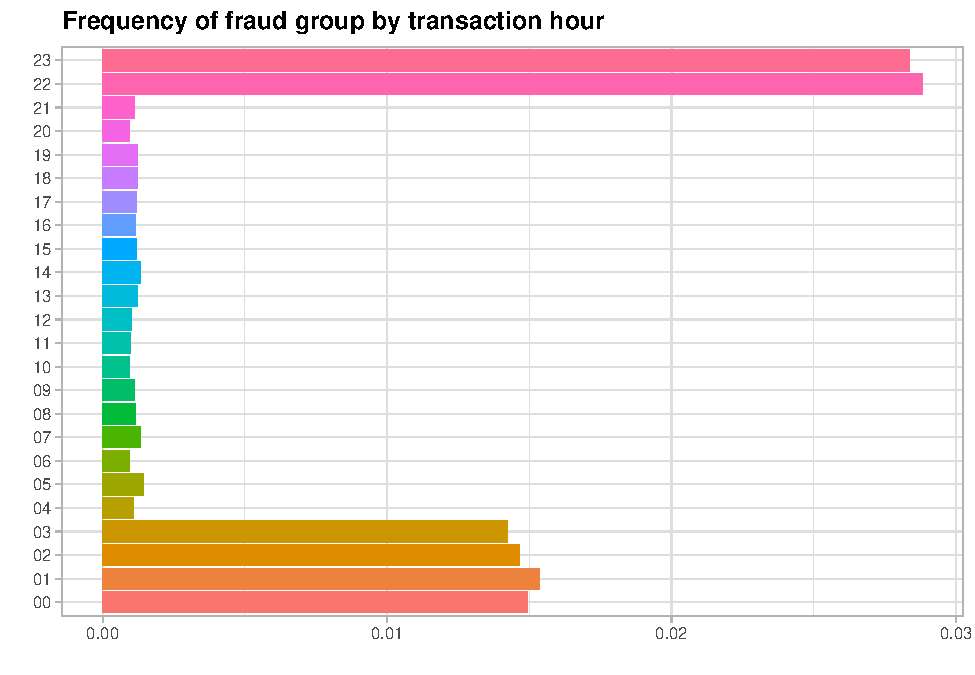
\includegraphics{credit_card_fraud_detection_files/figure-latex/hour_fraud_plot-1.pdf}
\caption{\label{Fig:hour_fraud_plot}Frequancy of fraudulent transactions
grouped by the transaction hour.}
\end{figure}

The analysis also shown, that month of a transaction is not very
important.

\hypertarget{distance}{%
\subsection{Distance}\label{distance}}

Now we will take a look at the distance between the home of a Holder and
the place of a Merchant. We will compute the distance based on
\texttt{lat}, \texttt{long}, \texttt{merch\_lat} and
\texttt{merch\_long} variables, that give us geo-coordinates for the
places, using the formula:
\[distance = \sqrt{(long-merch\ long)^2 + (lat-merch\ lat)^2}\]

\begin{Shaded}
\begin{Highlighting}[]
\NormalTok{data\_train[, dist }\SpecialCharTok{:}\ErrorTok{=} \FunctionTok{sqrt}\NormalTok{((long}\SpecialCharTok{{-}}\NormalTok{merch\_long)}\SpecialCharTok{\^{}}\DecValTok{2} \SpecialCharTok{+}\NormalTok{ (lat}\SpecialCharTok{{-}}\NormalTok{merch\_lat)}\SpecialCharTok{\^{}}\DecValTok{2}\NormalTok{)]}
\end{Highlighting}
\end{Shaded}

\begin{Shaded}
\begin{Highlighting}[]
\FunctionTok{ggplot}\NormalTok{(data\_train, }\FunctionTok{aes}\NormalTok{(}\AttributeTok{x =}\NormalTok{ is\_fraud, }\AttributeTok{y =}\NormalTok{ dist)) }\SpecialCharTok{+}
  \FunctionTok{geom\_boxplot}\NormalTok{() }\SpecialCharTok{+}
\NormalTok{  my\_style }\SpecialCharTok{+}
  \FunctionTok{labs}\NormalTok{(}\AttributeTok{title =} \StringTok{"Boxplot for distance between the home of a Holder and the place of a Merchant"}\NormalTok{,}
       \AttributeTok{subtitle =} \StringTok{"group by not{-}fraudulent transactions and fraudulent transactions"}\NormalTok{)}
\end{Highlighting}
\end{Shaded}

\begin{figure}
\centering
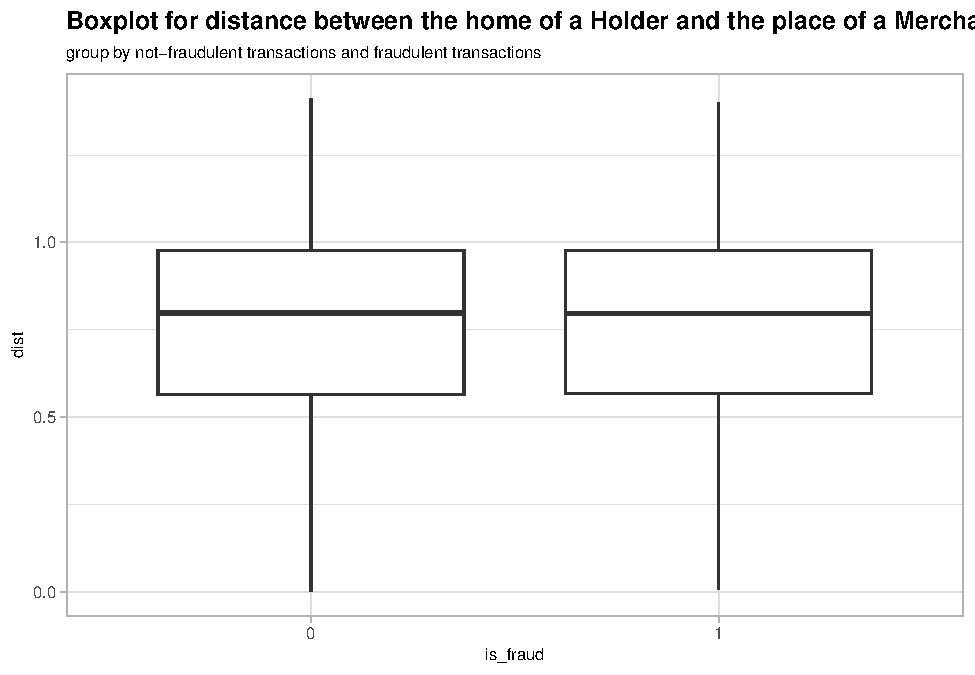
\includegraphics{credit_card_fraud_detection_files/figure-latex/dist_plot-1.pdf}
\caption{\label{Fig:dist_plot}Boxplot of distance between the home of a
Holder and the place of a Merchant, grouped by is\_fraud.}
\end{figure}

The boxplot shows no significant difference in distance for fraudulent
and non-fraudulent transactions.

\hypertarget{data-binning}{%
\section{Data binning}\label{data-binning}}

Keeping in mind the analysis described above, we will bin some
categorical variables, so that we have less categories (and less
variables in a model), but still have much information, that the columns
provide.

\hypertarget{information-value}{%
\subsection{Information Value}\label{information-value}}

We will perform binning with respect to Information Value and Weight of
Evidence provided by function \texttt{WOETable} form a package
\texttt{InformationValue} (code is based on the lecture materials).

\begin{Shaded}
\begin{Highlighting}[]
\NormalTok{categorical\_cols }\OtherTok{\textless{}{-}} \FunctionTok{c}\NormalTok{()}
\ControlFlowTok{for}\NormalTok{ (col }\ControlFlowTok{in} \FunctionTok{colnames}\NormalTok{(data\_train }\SpecialCharTok{\%\textgreater{}\%}\NormalTok{ .[, }\SpecialCharTok{{-}}\FunctionTok{c}\NormalTok{(}\StringTok{"cc\_num"}\NormalTok{, }\StringTok{"is\_fraud"}\NormalTok{)])) \{}
  
  \ControlFlowTok{if}\NormalTok{(}\FunctionTok{is.factor}\NormalTok{(data\_train[[col]])) \{}
\NormalTok{    categorical\_cols }\OtherTok{\textless{}{-}} \FunctionTok{c}\NormalTok{(categorical\_cols, col)}
\NormalTok{  \}}
  
\NormalTok{\}}

\NormalTok{woe\_table }\OtherTok{\textless{}{-}} \FunctionTok{woe}\NormalTok{(data\_train[, ..categorical\_cols], }
                 \FunctionTok{as.factor}\NormalTok{(data\_train}\SpecialCharTok{$}\NormalTok{is\_fraud),}
                 \AttributeTok{zeroadj =} \DecValTok{1}\NormalTok{)}
\end{Highlighting}
\end{Shaded}

\begin{verbatim}
## At least one empty cell (class x level) does exists. Zero adjustment applied!
## At least one empty cell (class x level) does exists. Zero adjustment applied!
## At least one empty cell (class x level) does exists. Zero adjustment applied!
## At least one empty cell (class x level) does exists. Zero adjustment applied!
\end{verbatim}

\begin{Shaded}
\begin{Highlighting}[]
\NormalTok{woe\_table}
\end{Highlighting}
\end{Shaded}

\begin{verbatim}
## Information values of transformed variables: 
## 
##                           IV
## trans_hour        1.86222611
## city              1.35711722
## merchant          0.86570833
## category          0.75817840
## job               0.69713416
## state             0.04938307
## week_day_of_trans 0.02518155
## gender            0.01008412
\end{verbatim}

\texttt{job}, \texttt{merchant}, \texttt{city} and \texttt{category}
seem to have high value, but they also have many categories (leading to
higher sum of IV). \texttt{gender} performs poorly and that is a little
bit surprising, giving the difference in fraud/non-fraud proportions.

Taking a look at the separate WOE tables for each variable, we can
conclude that particular jobs have low IV, the same can be observed for
\texttt{city}. For \texttt{category} the table looks better, we will
work with this variable and with \texttt{trans\_hour}. For
\texttt{state}, \texttt{week\_day\_trans} and \texttt{gender} the
results are rather poor, although we will try to work on the weekday of
transaction.

Now, we will apply the results combined with analysis of the plots shown
earlier and bin some variables.

\begin{Shaded}
\begin{Highlighting}[]
\NormalTok{data\_train[, weekday\_fraud }\SpecialCharTok{:}\ErrorTok{=} \FunctionTok{if\_else}\NormalTok{(week\_day\_of\_trans }\SpecialCharTok{\%in\%} \DecValTok{4}\SpecialCharTok{:}\DecValTok{7}\NormalTok{, }\DecValTok{1}\NormalTok{, }\DecValTok{0}\NormalTok{)]}
\NormalTok{data\_train[, category\_fraud }\SpecialCharTok{:}\ErrorTok{=} 
             \FunctionTok{if\_else}\NormalTok{(category }\SpecialCharTok{\%in\%} \FunctionTok{c}\NormalTok{(}\StringTok{\textquotesingle{}grocery\_pos\textquotesingle{}}\NormalTok{, }\StringTok{\textquotesingle{}misc\_net\textquotesingle{}}\NormalTok{, }\StringTok{\textquotesingle{}shopping\_net\textquotesingle{}}\NormalTok{, }\StringTok{\textquotesingle{}shopping\_pos\textquotesingle{}}\NormalTok{), }\DecValTok{1}\NormalTok{, }\DecValTok{0}\NormalTok{)]}
\NormalTok{data\_train[, hour\_fraud }\SpecialCharTok{:}\ErrorTok{=} 
             \FunctionTok{if\_else}\NormalTok{(trans\_hour }\SpecialCharTok{\%in\%} \FunctionTok{c}\NormalTok{(}\StringTok{\textquotesingle{}00\textquotesingle{}}\NormalTok{, }\StringTok{\textquotesingle{}01\textquotesingle{}}\NormalTok{, }\StringTok{\textquotesingle{}02\textquotesingle{}}\NormalTok{, }\StringTok{\textquotesingle{}03\textquotesingle{}}\NormalTok{, }\StringTok{\textquotesingle{}22\textquotesingle{}}\NormalTok{, }\StringTok{\textquotesingle{}23\textquotesingle{}}\NormalTok{), }\DecValTok{1}\NormalTok{, }\DecValTok{0}\NormalTok{)]}
\NormalTok{data\_train[,}\FunctionTok{c}\NormalTok{(}\StringTok{"weekday\_fraud"}\NormalTok{, }\StringTok{"category\_fraud"}\NormalTok{, }\StringTok{"hour\_fraud"}\NormalTok{)}\SpecialCharTok{:}\ErrorTok{=} 
             \FunctionTok{lapply}\NormalTok{(.SD, as.factor), .SDcols }\OtherTok{=} \FunctionTok{c}\NormalTok{(}\StringTok{"weekday\_fraud"}\NormalTok{, }\StringTok{"category\_fraud"}\NormalTok{, }\StringTok{"hour\_fraud"}\NormalTok{)]}
\end{Highlighting}
\end{Shaded}

We can also drop more variables (for binned and unbinned data):

\begin{itemize}
\tightlist
\item
  lat, long, merch\_lat, merch\_long - beacause they were used to create
  \texttt{dist} and we do not need them anymore,
\item
  cc\_num - we will not use credit card number,
\item
  merchant - there are too many categories (693),
\item
  dob - date of birth of a Holder will not be used, as we have created
  the age variable,
\item
  trans\_date\_trans\_time - was needed only to create
  \texttt{trans\_hour}.
\end{itemize}

Also, we will add binned variables to \texttt{data}, because we will
perform normalization and our data is too big to keep all three datasets
with original, binned and normalized data.

\hypertarget{normalization}{%
\section{Normalization}\label{normalization}}

As mentioned before, we will not create another dataset with unbinned
and normalized data, because it is too big and takes too much memory to
keep it. So let us normalize \texttt{data\_bin} and leave \texttt{data}
in its original ranges.

To perform normalization, we will use a function \texttt{min\_max\_norm}
from lecture materials.

\begin{Shaded}
\begin{Highlighting}[]
\NormalTok{min\_max\_norm }\OtherTok{\textless{}{-}} \ControlFlowTok{function}\NormalTok{(x) \{}
\NormalTok{  (x }\SpecialCharTok{{-}} \FunctionTok{min}\NormalTok{(x, }\AttributeTok{na.rm =}\NormalTok{ T)) }\SpecialCharTok{/}\NormalTok{ (}\FunctionTok{max}\NormalTok{(x, }\AttributeTok{na.rm =}\NormalTok{ T) }\SpecialCharTok{{-}} \FunctionTok{min}\NormalTok{(x, }\AttributeTok{na.rm =}\NormalTok{ T))}
\NormalTok{\}}

\NormalTok{temp }\OtherTok{\textless{}{-}} \FunctionTok{c}\NormalTok{(}\StringTok{\textquotesingle{}amt\textquotesingle{}}\NormalTok{,}\StringTok{\textquotesingle{}city\_pop\textquotesingle{}}\NormalTok{,}\StringTok{\textquotesingle{}age\textquotesingle{}}\NormalTok{,}\StringTok{\textquotesingle{}dist\textquotesingle{}}\NormalTok{)}
\NormalTok{data\_train\_bin }\OtherTok{\textless{}{-}} \FunctionTok{copy}\NormalTok{(data\_train)}
\NormalTok{data\_train\_bin[, (temp) }\SpecialCharTok{:}\ErrorTok{=} \FunctionTok{lapply}\NormalTok{(.SD, min\_max\_norm), .SDcols }\OtherTok{=}\NormalTok{ temp] }\CommentTok{\# reference!}
\end{Highlighting}
\end{Shaded}

\hypertarget{correlation}{%
\section{Correlation}\label{correlation}}

\begin{Shaded}
\begin{Highlighting}[]
\FunctionTok{ggcorr}\NormalTok{(data\_train[, ..temp], }\AttributeTok{label =}\NormalTok{ T)}
\end{Highlighting}
\end{Shaded}

\begin{figure}
\centering
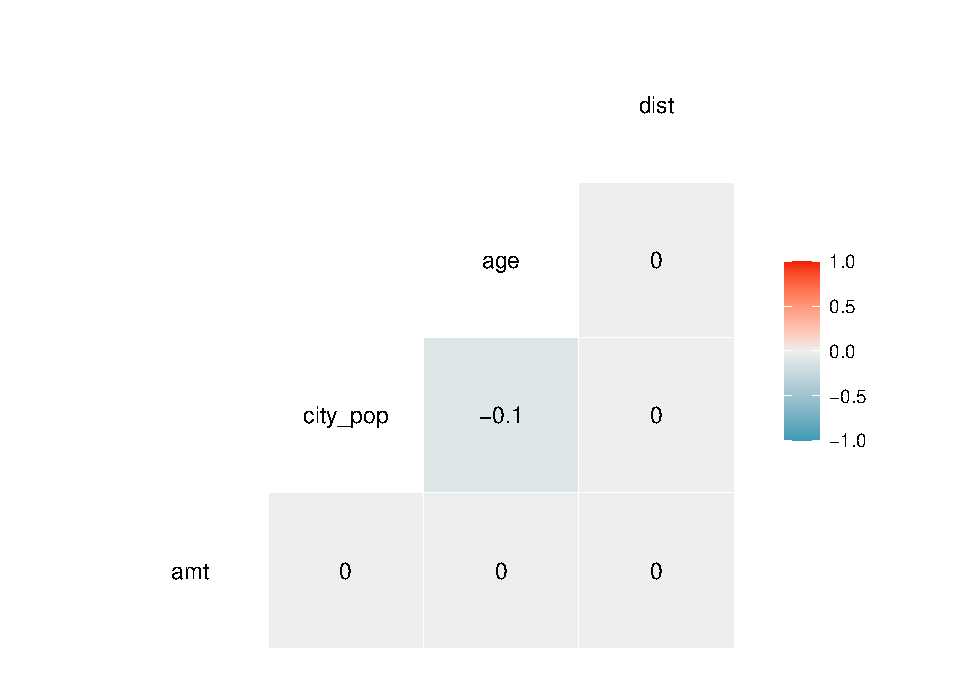
\includegraphics{credit_card_fraud_detection_files/figure-latex/correlation-1.pdf}
\caption{The correlation structure of the data.}
\end{figure}

Correlation is very low for all numerical variables.

\hypertarget{models}{%
\chapter{Models}\label{models}}

\hypertarget{cross-validation}{%
\section{Cross Validation}\label{cross-validation}}

To investigate how well the model is dealing with new datapoints we set
20\% of the data aside for cross validation. We make it on both datasets
with normalized data and not-normalized data.

\begin{Shaded}
\begin{Highlighting}[]
\FunctionTok{set.seed}\NormalTok{(}\DecValTok{125}\NormalTok{)}
\NormalTok{data\_train\_bin\_cv }\OtherTok{\textless{}{-}} \FunctionTok{resample\_partition}\NormalTok{(data\_train\_bin, }\AttributeTok{p =} \FunctionTok{c}\NormalTok{(}\AttributeTok{valid =} \FloatTok{0.3}\NormalTok{, }\AttributeTok{train =} \FloatTok{0.7}\NormalTok{))}
\NormalTok{train\_bin\_cv }\OtherTok{\textless{}{-}}\NormalTok{ data\_train\_bin[data\_train\_bin\_cv}\SpecialCharTok{$}\NormalTok{train}\SpecialCharTok{$}\NormalTok{idx,]}
\NormalTok{valid\_bin\_cv }\OtherTok{\textless{}{-}}\NormalTok{ data\_train\_bin[data\_train\_bin\_cv}\SpecialCharTok{$}\NormalTok{valid}\SpecialCharTok{$}\NormalTok{idx,]}
\end{Highlighting}
\end{Shaded}

\hypertarget{the-base-model}{%
\section{The base model}\label{the-base-model}}

\hypertarget{logistic-regression}{%
\subsection{Logistic regression}\label{logistic-regression}}

As a base model we will consider logistic regression with variables
which give the best results after investigation.

\begin{Shaded}
\begin{Highlighting}[]
\NormalTok{logreg }\OtherTok{\textless{}{-}} \FunctionTok{glm}\NormalTok{(is\_fraud }\SpecialCharTok{\textasciitilde{}} 
\NormalTok{                category\_fraud }\SpecialCharTok{+}\NormalTok{ amt }\SpecialCharTok{+}\NormalTok{ hour\_fraud }\SpecialCharTok{+}\NormalTok{ age}\SpecialCharTok{:}\NormalTok{hour\_fraud }\SpecialCharTok{+}\NormalTok{ amt}\SpecialCharTok{:}\NormalTok{hour\_fraud }\SpecialCharTok{+} 
\NormalTok{                amt}\SpecialCharTok{:}\NormalTok{category\_fraud }\SpecialCharTok{+}\NormalTok{ age}\SpecialCharTok{:}\NormalTok{category\_fraud,}
              \AttributeTok{data =}\NormalTok{ train\_bin\_cv, }\AttributeTok{family =}\NormalTok{ binomial)}
\FunctionTok{summary}\NormalTok{(logreg)}
\end{Highlighting}
\end{Shaded}

\begin{verbatim}
## 
## Call:
## glm(formula = is_fraud ~ category_fraud + amt + hour_fraud + 
##     age:hour_fraud + amt:hour_fraud + amt:category_fraud + age:category_fraud, 
##     family = binomial, data = train_bin_cv)
## 
## Deviance Residuals: 
##     Min       1Q   Median       3Q      Max  
## -8.4904  -0.0711  -0.0443  -0.0392   4.4390  
## 
## Coefficients:
##                      Estimate Std. Error z value Pr(>|z|)    
## (Intercept)          -7.26220    0.08810 -82.427  < 2e-16 ***
## category_fraud1      -0.41384    0.07493  -5.523 3.33e-08 ***
## amt                 -85.53658    3.32968 -25.689  < 2e-16 ***
## hour_fraud1           2.67919    0.09282  28.864  < 2e-16 ***
## hour_fraud0:age       0.85232    0.17545   4.858 1.19e-06 ***
## hour_fraud1:age      -0.42094    0.12624  -3.334 0.000855 ***
## amt:hour_fraud1     107.92782    2.37217  45.498  < 2e-16 ***
## category_fraud1:amt 146.98121    2.98194  49.290  < 2e-16 ***
## category_fraud1:age   1.26192    0.15201   8.301  < 2e-16 ***
## ---
## Signif. codes:  0 '***' 0.001 '**' 0.01 '*' 0.05 '.' 0.1 ' ' 1
## 
## (Dispersion parameter for binomial family taken to be 1)
## 
##     Null deviance: 64850  on 907672  degrees of freedom
## Residual deviance: 41229  on 907664  degrees of freedom
## AIC: 41247
## 
## Number of Fisher Scoring iterations: 9
\end{verbatim}

We would like to point out that we are focusing on maximizing recall,
but also try to keep precision on a reasonable level. To check the model
we created a function which computes a confusion matrix and also gives
us values for recall and precision.

\begin{Shaded}
\begin{Highlighting}[]
\NormalTok{confusion\_matrix }\OtherTok{\textless{}{-}} \ControlFlowTok{function}\NormalTok{(model, data, col, }\AttributeTok{cutoff=}\FloatTok{0.5}\NormalTok{, }\AttributeTok{model\_type =} \StringTok{"logistic"}\NormalTok{) \{}
  
\NormalTok{  predictScore }\OtherTok{\textless{}{-}} \FunctionTok{as.numeric}\NormalTok{(}\FunctionTok{predict}\NormalTok{(}\AttributeTok{object=}\NormalTok{model, }\AttributeTok{type=}\StringTok{\textquotesingle{}response\textquotesingle{}}\NormalTok{,}\AttributeTok{newdat=}\NormalTok{data)) }\CommentTok{\# calculating prediction scores}
  
  \ControlFlowTok{if}\NormalTok{ (model\_type }\SpecialCharTok{==} \StringTok{"forest"}\NormalTok{) predictScore }\OtherTok{=}\NormalTok{ predictScore }\SpecialCharTok{{-}}\DecValTok{1}
  
\NormalTok{  predic }\OtherTok{\textless{}{-}} \FunctionTok{if\_else}\NormalTok{(predictScore }\SpecialCharTok{\textgreater{}}\NormalTok{ cutoff, }\DecValTok{1}\NormalTok{, }\DecValTok{0}\NormalTok{) }\CommentTok{\# assigning predictions}
\NormalTok{  confmat }\OtherTok{\textless{}{-}} \FunctionTok{table}\NormalTok{(predic, data[[col]])}
  
  \FunctionTok{rownames}\NormalTok{(confmat) }\OtherTok{\textless{}{-}} \FunctionTok{c}\NormalTok{(}\StringTok{\textquotesingle{}pred\_negative\textquotesingle{}}\NormalTok{, }\StringTok{\textquotesingle{}pred\_positive\textquotesingle{}}\NormalTok{)}
  \FunctionTok{colnames}\NormalTok{(confmat) }\OtherTok{\textless{}{-}} \FunctionTok{c}\NormalTok{(}\StringTok{\textquotesingle{}obs\_negative\textquotesingle{}}\NormalTok{, }\StringTok{\textquotesingle{}obs\_positive\textquotesingle{}}\NormalTok{)}
  
\NormalTok{  precision }\OtherTok{\textless{}{-}}\NormalTok{ confmat[}\DecValTok{2}\NormalTok{,}\DecValTok{2}\NormalTok{]}\SpecialCharTok{/}\NormalTok{(confmat[}\DecValTok{2}\NormalTok{,}\DecValTok{1}\NormalTok{]}\SpecialCharTok{+}\NormalTok{confmat[}\DecValTok{2}\NormalTok{,}\DecValTok{2}\NormalTok{]) }\CommentTok{\# precision = TP/(TP+FP)}
\NormalTok{  recall }\OtherTok{\textless{}{-}}\NormalTok{ confmat[}\DecValTok{2}\NormalTok{,}\DecValTok{2}\NormalTok{]}\SpecialCharTok{/}\NormalTok{(confmat[}\DecValTok{1}\NormalTok{,}\DecValTok{2}\NormalTok{]}\SpecialCharTok{+}\NormalTok{confmat[}\DecValTok{2}\NormalTok{,}\DecValTok{2}\NormalTok{]) }\CommentTok{\# recall = TP/(TP+FN)}
  
  \FunctionTok{return}\NormalTok{(}\FunctionTok{c}\NormalTok{(precision, recall))}
\NormalTok{\}}
\end{Highlighting}
\end{Shaded}

To fit the best model we create a function which produces a plot for
precision and recall for each model by changing the value of parameter
\texttt{cutoff} in the \texttt{glm} function.

\begin{Shaded}
\begin{Highlighting}[]
\CommentTok{\# looking for the most reasonable cutoff for a model {-} the function produces a plot}
\NormalTok{find\_cutoff }\OtherTok{\textless{}{-}} \ControlFlowTok{function}\NormalTok{(model, data, target\_variable, }\AttributeTok{min\_cutoff=}\FloatTok{0.1}\NormalTok{, }\AttributeTok{max\_cutoff=}\FloatTok{0.8}\NormalTok{, }\AttributeTok{by=}\FloatTok{0.05}\NormalTok{)\{}
\NormalTok{  cutoffs }\OtherTok{\textless{}{-}} \FunctionTok{seq}\NormalTok{(min\_cutoff, max\_cutoff, }\AttributeTok{by=}\NormalTok{by)}
\NormalTok{  precisions }\OtherTok{\textless{}{-}} \FunctionTok{numeric}\NormalTok{(}\DecValTok{0}\NormalTok{)}
\NormalTok{  recalls }\OtherTok{\textless{}{-}} \FunctionTok{numeric}\NormalTok{(}\DecValTok{0}\NormalTok{)}
  \ControlFlowTok{for}\NormalTok{(x }\ControlFlowTok{in}\NormalTok{ cutoffs)\{}
    \CommentTok{\# confusion matrix for the model with cutoff = x}
\NormalTok{    conf\_mat }\OtherTok{\textless{}{-}} \FunctionTok{confusion\_matrix}\NormalTok{(model, data, target\_variable, x) }
\NormalTok{    precisions }\OtherTok{\textless{}{-}} \FunctionTok{c}\NormalTok{(precisions, conf\_mat[}\DecValTok{1}\NormalTok{])}
\NormalTok{    recalls }\OtherTok{\textless{}{-}} \FunctionTok{c}\NormalTok{(recalls, conf\_mat[}\DecValTok{2}\NormalTok{])}
\NormalTok{  \}}
  \CommentTok{\# preparation for a plot}
\NormalTok{  metrics }\OtherTok{\textless{}{-}} \FunctionTok{tibble}\NormalTok{(}
    \AttributeTok{cutoffs =}\NormalTok{ cutoffs,}
    \AttributeTok{precisions =}\NormalTok{ precisions,}
    \AttributeTok{recalls =}\NormalTok{ recalls}
\NormalTok{  )}
\NormalTok{  metrics\_long }\OtherTok{\textless{}{-}} \FunctionTok{melt}\NormalTok{(metrics, }\AttributeTok{id=}\StringTok{\textquotesingle{}cutoffs\textquotesingle{}}\NormalTok{)}
\NormalTok{  pl }\OtherTok{\textless{}{-}} \FunctionTok{ggplot}\NormalTok{(}\AttributeTok{data=}\NormalTok{metrics\_long, }\FunctionTok{aes}\NormalTok{(}\AttributeTok{x=}\NormalTok{cutoffs, }\AttributeTok{y=}\NormalTok{value, }\AttributeTok{colour=}\NormalTok{variable)) }\SpecialCharTok{+} 
    \FunctionTok{geom\_line}\NormalTok{(}\AttributeTok{size=}\DecValTok{1}\NormalTok{) }\SpecialCharTok{+}
    \FunctionTok{scale\_colour\_discrete}\NormalTok{(}\AttributeTok{name  =}\StringTok{"Metric"}\NormalTok{,}
                          \AttributeTok{breaks=}\FunctionTok{c}\NormalTok{(}\StringTok{"precisions"}\NormalTok{, }\StringTok{"recalls"}\NormalTok{),}
                          \AttributeTok{labels=}\FunctionTok{c}\NormalTok{(}\StringTok{"Precision"}\NormalTok{, }\StringTok{"Recall"}\NormalTok{)) }\SpecialCharTok{+}
    \FunctionTok{labs}\NormalTok{(}\AttributeTok{title=}\StringTok{\textquotesingle{}Precision \& recall rates\textquotesingle{}}\NormalTok{,}
         \AttributeTok{subtitle=}\StringTok{\textquotesingle{}as functions of the cutoff\textquotesingle{}}\NormalTok{,}
         \AttributeTok{x=}\StringTok{\textquotesingle{}Cutoff\textquotesingle{}}\NormalTok{, }\AttributeTok{y=}\StringTok{\textquotesingle{}\textquotesingle{}}\NormalTok{) }\SpecialCharTok{+}
   \FunctionTok{theme\_light}\NormalTok{() }\SpecialCharTok{+}
    \FunctionTok{theme}\NormalTok{(}
      \AttributeTok{plot.subtitle =} \FunctionTok{element\_text}\NormalTok{(}\AttributeTok{size =}\NormalTok{ text\_size }\SpecialCharTok{{-}} \DecValTok{4}\NormalTok{, }\AttributeTok{colour=}\StringTok{\textquotesingle{}black\textquotesingle{}}\NormalTok{),}
      \AttributeTok{plot.title =} \FunctionTok{element\_text}\NormalTok{(}\AttributeTok{size =}\NormalTok{ text\_size, }\AttributeTok{face =} \StringTok{\textquotesingle{}bold\textquotesingle{}}\NormalTok{),}
      \AttributeTok{axis.text=}\FunctionTok{element\_text}\NormalTok{(}\AttributeTok{size=}\NormalTok{text\_size }\SpecialCharTok{{-}} \DecValTok{4}\NormalTok{), }
      \AttributeTok{axis.title.y =} \FunctionTok{element\_text}\NormalTok{(}\AttributeTok{size =}\NormalTok{ text\_size }\SpecialCharTok{{-}} \DecValTok{4}\NormalTok{), }
      \AttributeTok{axis.title.x =} \FunctionTok{element\_text}\NormalTok{(}\AttributeTok{size =}\NormalTok{ text\_size }\SpecialCharTok{{-}} \DecValTok{4}\NormalTok{),}
      \AttributeTok{legend.position =} \FunctionTok{c}\NormalTok{(}\FloatTok{0.9}\NormalTok{,}\FloatTok{0.9}\NormalTok{)}
\NormalTok{    )}
  \CommentTok{\# plotting}
  \FunctionTok{grid.arrange}\NormalTok{(pl, }\AttributeTok{nrow=}\DecValTok{1}\NormalTok{, }\AttributeTok{ncol=}\DecValTok{1}\NormalTok{)}
  
\NormalTok{\}}
\end{Highlighting}
\end{Shaded}

\begin{Shaded}
\begin{Highlighting}[]
\FunctionTok{find\_cutoff}\NormalTok{(logreg, train\_bin\_cv, }\StringTok{\textquotesingle{}is\_fraud\textquotesingle{}}\NormalTok{, }\FloatTok{0.001}\NormalTok{, }\FloatTok{0.1}\NormalTok{, }\FloatTok{0.001}\NormalTok{)}
\end{Highlighting}
\end{Shaded}

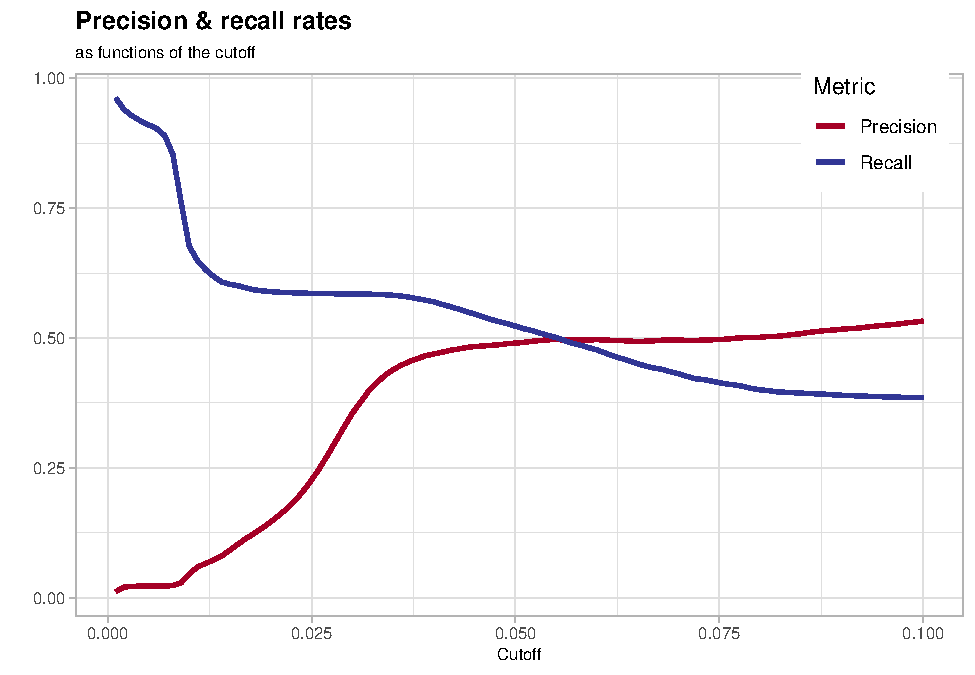
\includegraphics{credit_card_fraud_detection_files/figure-latex/cutoff_lvl-1.pdf}
The function creates a graph, where we can we pick up a parameter
optimal for us. We will go for value \texttt{0.03} as the best cutoff
level which maximizes recall.

Let us look at the confusion matrix:

\begin{Shaded}
\begin{Highlighting}[]
\NormalTok{conf\_mat\_logreg\_train }\OtherTok{\textless{}{-}} 
  \FunctionTok{confusion\_matrix}\NormalTok{(logreg, train\_bin\_cv, }\AttributeTok{col =} \StringTok{"is\_fraud"}\NormalTok{, }\AttributeTok{cutoff =} \FloatTok{0.003}\NormalTok{)}
\NormalTok{conf\_mat\_logreg\_valid }\OtherTok{\textless{}{-}} 
  \FunctionTok{confusion\_matrix}\NormalTok{(logreg, valid\_bin\_cv, }\AttributeTok{col =} \StringTok{"is\_fraud"}\NormalTok{, }\AttributeTok{cutoff =} \FloatTok{0.003}\NormalTok{)}
\NormalTok{conf\_mat\_logreg\_train}
\end{Highlighting}
\end{Shaded}

\begin{verbatim}
## [1] 0.02168837 0.92761038
\end{verbatim}

\begin{Shaded}
\begin{Highlighting}[]
\NormalTok{conf\_mat\_logreg\_valid}
\end{Highlighting}
\end{Shaded}

\begin{verbatim}
## [1] 0.02137988 0.92866756
\end{verbatim}

As a result we get on training dataset precision equals 0.022, recall
equals 0.928 and on testing dataset precision equals 0.021, recall
equals 0.929. This model is a good contender, but in next consideration
we will focus on getting higher precision with assuming high recall.

\hypertarget{the-challenger-models}{%
\section{The Challenger models}\label{the-challenger-models}}

\hypertarget{logistic-regression-with-pca}{%
\subsection{Logistic regression with
PCA}\label{logistic-regression-with-pca}}

First challenger model will be a logistic regression with application of
Principal Component Analysis (PCA) on numerical variables.

\begin{Shaded}
\begin{Highlighting}[]
\CommentTok{\# remove dependent variable from dataset and keep only numerical variables}
\NormalTok{numerical\_cols }\OtherTok{\textless{}{-}} \FunctionTok{c}\NormalTok{(}\StringTok{\textquotesingle{}amt\textquotesingle{}}\NormalTok{, }\StringTok{\textquotesingle{}city\_pop\textquotesingle{}}\NormalTok{, }\StringTok{\textquotesingle{}age\textquotesingle{}}\NormalTok{, }\StringTok{\textquotesingle{}dist\textquotesingle{}}\NormalTok{, }\StringTok{\textquotesingle{}weekday\_fraud\textquotesingle{}}\NormalTok{, }\StringTok{\textquotesingle{}category\_fraud\textquotesingle{}}\NormalTok{, }\StringTok{\textquotesingle{}hour\_fraud\textquotesingle{}}\NormalTok{)}
\NormalTok{data\_bin\_PCA }\OtherTok{\textless{}{-}}\NormalTok{ data\_train\_bin }\SpecialCharTok{\%\textgreater{}\%} 
\NormalTok{  .[, (numerical\_cols)}\SpecialCharTok{:}\ErrorTok{=} \FunctionTok{lapply}\NormalTok{(.SD, as.numeric), .SDcols }\OtherTok{=}\NormalTok{ numerical\_cols] }\SpecialCharTok{\%\textgreater{}\%}
\NormalTok{  .[, ..numerical\_cols]}

\CommentTok{\# the PCA analysis:}
\NormalTok{pca\_decomposition }\OtherTok{\textless{}{-}} \FunctionTok{prcomp}\NormalTok{(data\_bin\_PCA)}
\end{Highlighting}
\end{Shaded}

Calculate a percentage of variance explained by each PCA component.

\begin{Shaded}
\begin{Highlighting}[]
\CommentTok{\# calculating a variance of each component}
\NormalTok{variance }\OtherTok{\textless{}{-}}\NormalTok{ pca\_decomposition}\SpecialCharTok{$}\NormalTok{sdev}\SpecialCharTok{\^{}}\DecValTok{2}
\NormalTok{variance\_perc }\OtherTok{\textless{}{-}} \FunctionTok{round}\NormalTok{(variance}\SpecialCharTok{/}\FunctionTok{sum}\NormalTok{(variance),}\DecValTok{4}\NormalTok{)}
\end{Highlighting}
\end{Shaded}

\begin{Shaded}
\begin{Highlighting}[]
\FunctionTok{ggplot}\NormalTok{(}\AttributeTok{data =} \FunctionTok{as.data.frame}\NormalTok{(variance\_perc), }
       \FunctionTok{aes}\NormalTok{(}\AttributeTok{x =} \FunctionTok{paste0}\NormalTok{(}\StringTok{\textquotesingle{}PC\textquotesingle{}}\NormalTok{, }\DecValTok{1}\SpecialCharTok{:}\DecValTok{7}\NormalTok{), }\AttributeTok{y =}\NormalTok{ variance\_perc)) }\SpecialCharTok{+}
  \FunctionTok{geom\_col}\NormalTok{() }\SpecialCharTok{+}
  \FunctionTok{xlab}\NormalTok{(}\StringTok{""}\NormalTok{) }\SpecialCharTok{+} 
  \FunctionTok{labs}\NormalTok{(}\AttributeTok{title=} \StringTok{\textquotesingle{}Variance\textquotesingle{}}\NormalTok{, }\AttributeTok{subtitle=}\StringTok{\textquotesingle{}for each PCs\textquotesingle{}}\NormalTok{,}\AttributeTok{x=}\StringTok{\textquotesingle{}\textquotesingle{}}\NormalTok{, }\AttributeTok{y=}\StringTok{\textquotesingle{}\textquotesingle{}}\NormalTok{) }\SpecialCharTok{+}
\NormalTok{  my\_style}
\end{Highlighting}
\end{Shaded}

\begin{figure}
\centering
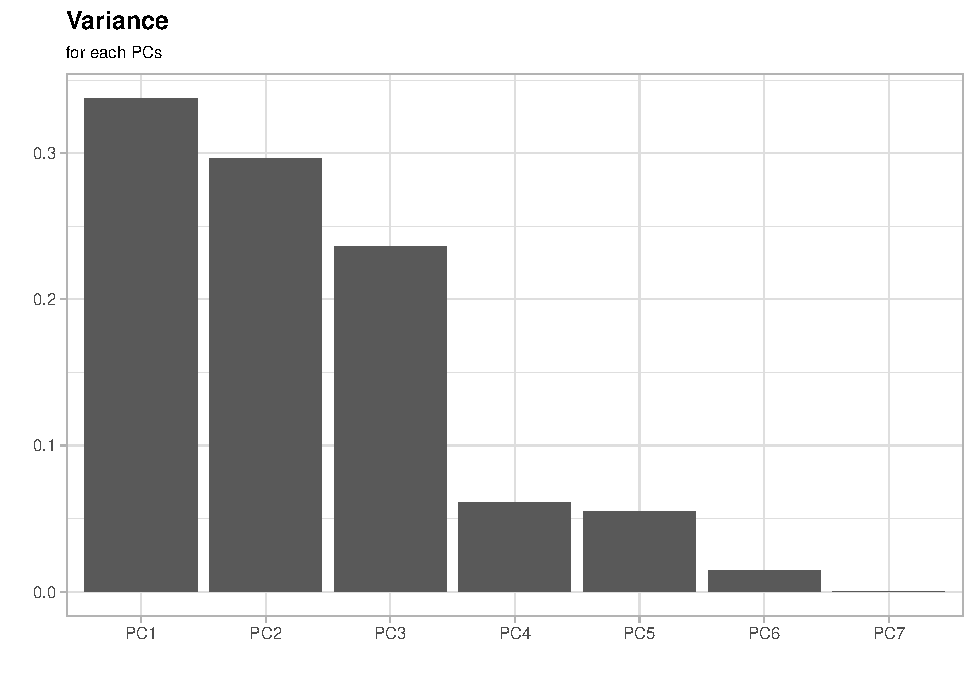
\includegraphics{credit_card_fraud_detection_files/figure-latex/pca_plot-1.pdf}
\caption{\label{Fig:pca_plot}Variance for each PCs}
\end{figure}

As we can see first three components account the most of the variance of
the data, but the third component could be also valuable for a model.

\begin{Shaded}
\begin{Highlighting}[]
\NormalTok{data\_train\_pca }\OtherTok{\textless{}{-}} \FunctionTok{cbind}\NormalTok{(data\_train}\SpecialCharTok{$}\NormalTok{is\_fraud, }\FunctionTok{as.data.table}\NormalTok{(pca\_decomposition}\SpecialCharTok{$}\NormalTok{x)) }\SpecialCharTok{\%\textgreater{}\%}
  \FunctionTok{setNames}\NormalTok{(}\FunctionTok{c}\NormalTok{(}\StringTok{"is\_fraud"}\NormalTok{, }\FunctionTok{paste0}\NormalTok{(}\StringTok{"PC"}\NormalTok{, }\DecValTok{1}\SpecialCharTok{:}\DecValTok{7}\NormalTok{)))}
\end{Highlighting}
\end{Shaded}

\begin{Shaded}
\begin{Highlighting}[]
\NormalTok{train\_bin\_cv\_pca }\OtherTok{\textless{}{-}}\NormalTok{ data\_train\_pca[data\_train\_bin\_cv}\SpecialCharTok{$}\NormalTok{train}\SpecialCharTok{$}\NormalTok{idx,]}
\NormalTok{valid\_bin\_cv\_pca }\OtherTok{\textless{}{-}}\NormalTok{ data\_train\_pca[data\_train\_bin\_cv}\SpecialCharTok{$}\NormalTok{valid}\SpecialCharTok{$}\NormalTok{idx,]}
\end{Highlighting}
\end{Shaded}

\begin{Shaded}
\begin{Highlighting}[]
\NormalTok{logreg\_PCA }\OtherTok{\textless{}{-}} \FunctionTok{glm}\NormalTok{(is\_fraud }\SpecialCharTok{\textasciitilde{}} 
\NormalTok{                    PC1 }\SpecialCharTok{+}\NormalTok{ PC2 }\SpecialCharTok{+}\NormalTok{ PC3 }\SpecialCharTok{+}\NormalTok{ PC4 }\SpecialCharTok{+}\NormalTok{ PC2}\SpecialCharTok{*}\NormalTok{PC3 }\SpecialCharTok{+}\NormalTok{ PC1}\SpecialCharTok{*}\NormalTok{PC4,}
                  \AttributeTok{data =}\NormalTok{ train\_bin\_cv\_pca, }\AttributeTok{family =}\NormalTok{ binomial)}
\FunctionTok{summary}\NormalTok{(logreg\_PCA)}
\end{Highlighting}
\end{Shaded}

\begin{verbatim}
## 
## Call:
## glm(formula = is_fraud ~ PC1 + PC2 + PC3 + PC4 + PC2 * PC3 + 
##     PC1 * PC4, family = binomial, data = train_bin_cv_pca)
## 
## Deviance Residuals: 
##     Min       1Q   Median       3Q      Max  
## -0.3642  -0.0834  -0.0368  -0.0307   3.9304  
## 
## Coefficients:
##             Estimate Std. Error  z value Pr(>|z|)    
## (Intercept) -6.37772    0.03539 -180.202  < 2e-16 ***
## PC1          0.26176    0.02819    9.286  < 2e-16 ***
## PC2         -2.46283    0.05994  -41.086  < 2e-16 ***
## PC3          2.25544    0.05020   44.930  < 2e-16 ***
## PC4         -0.32419    0.06483   -5.000 5.73e-07 ***
## PC2:PC3      0.39741    0.10803    3.679 0.000235 ***
## PC1:PC4     -0.59818    0.12892   -4.640 3.48e-06 ***
## ---
## Signif. codes:  0 '***' 0.001 '**' 0.01 '*' 0.05 '.' 0.1 ' ' 1
## 
## (Dispersion parameter for binomial family taken to be 1)
## 
##     Null deviance: 64850  on 907672  degrees of freedom
## Residual deviance: 53341  on 907666  degrees of freedom
## AIC: 53355
## 
## Number of Fisher Scoring iterations: 10
\end{verbatim}

\begin{Shaded}
\begin{Highlighting}[]
\FunctionTok{find\_cutoff}\NormalTok{(logreg\_PCA, train\_bin\_cv\_pca, }\StringTok{\textquotesingle{}is\_fraud\textquotesingle{}}\NormalTok{, }\FloatTok{0.001}\NormalTok{, }\FloatTok{0.05}\NormalTok{, }\FloatTok{0.001}\NormalTok{)}
\end{Highlighting}
\end{Shaded}

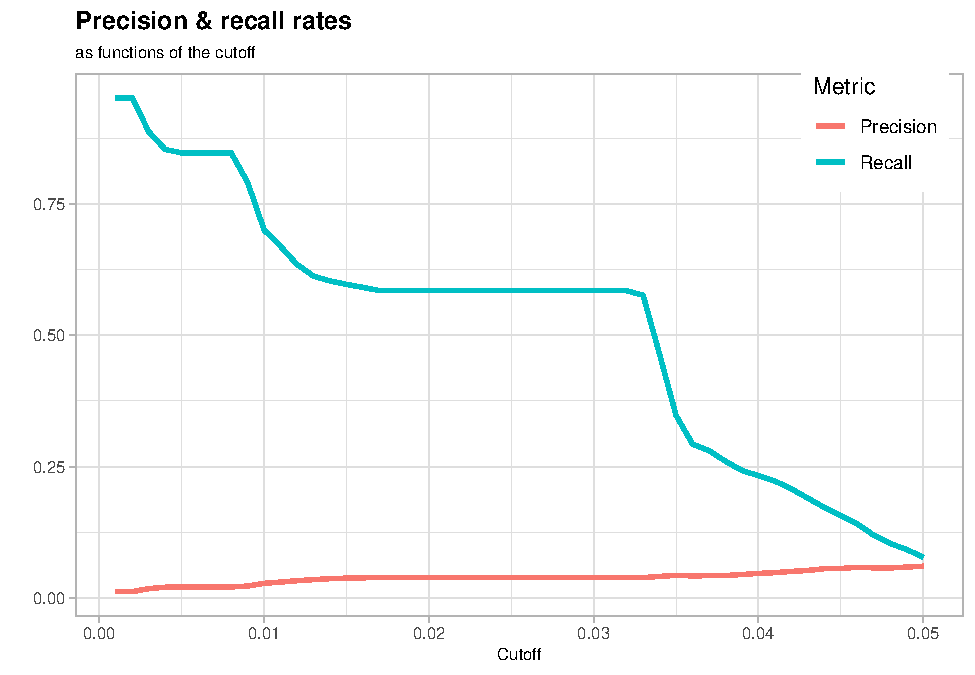
\includegraphics{credit_card_fraud_detection_files/figure-latex/logreg_PCA-1.pdf}

\begin{Shaded}
\begin{Highlighting}[]
\NormalTok{conf\_mat\_logreg\_PCA\_train }\OtherTok{\textless{}{-}} 
  \FunctionTok{confusion\_matrix}\NormalTok{(logreg\_PCA, train\_bin\_cv\_pca, }\AttributeTok{col =} \StringTok{"is\_fraud"}\NormalTok{, }\AttributeTok{cutoff =} \FloatTok{0.0025}\NormalTok{)}
\NormalTok{conf\_mat\_logreg\_PCA\_valid }\OtherTok{\textless{}{-}} 
  \FunctionTok{confusion\_matrix}\NormalTok{(logreg\_PCA, valid\_bin\_cv\_pca, }\AttributeTok{col =} \StringTok{"is\_fraud"}\NormalTok{, }\AttributeTok{cutoff =} \FloatTok{0.0025}\NormalTok{)}
\NormalTok{conf\_mat\_logreg\_PCA\_train}
\end{Highlighting}
\end{Shaded}

\begin{verbatim}
## [1] 0.01537381 0.90449119
\end{verbatim}

\begin{Shaded}
\begin{Highlighting}[]
\NormalTok{conf\_mat\_logreg\_PCA\_valid}
\end{Highlighting}
\end{Shaded}

\begin{verbatim}
## [1] 0.01523636 0.90937640
\end{verbatim}

As a result we get on training dataset precision = 0.015, recall = 0.904
and on testing dataset precision = 0.015, recall = 0.909.

For that model we have similar results as for the previous logistic
model. Moreover, we lose interpretation for numerical variables.

\hypertarget{random-forest}{%
\subsection{Random Forest}\label{random-forest}}

First, we need to create a train-test split on unnormalized data. As it
was before, we use 80\% of our data as a training set and 20\% as a
testing set.

\begin{Shaded}
\begin{Highlighting}[]
\NormalTok{train\_cv }\OtherTok{\textless{}{-}}\NormalTok{ data\_train[data\_train\_bin\_cv}\SpecialCharTok{$}\NormalTok{train}\SpecialCharTok{$}\NormalTok{idx,]}
\NormalTok{valid\_cv }\OtherTok{\textless{}{-}}\NormalTok{ data\_train[data\_train\_bin\_cv}\SpecialCharTok{$}\NormalTok{valid}\SpecialCharTok{$}\NormalTok{idx,]}
\end{Highlighting}
\end{Shaded}

As our data is highly imbalanced, we need to find optimal parameters for
a random forest in order to fit the model that performs well. To find
this parameter we will use a function called \texttt{find\_classwt}:

\begin{Shaded}
\begin{Highlighting}[]
\NormalTok{find\_classwt }\OtherTok{\textless{}{-}} \ControlFlowTok{function}\NormalTok{(data) \{}
  
\NormalTok{  recalls }\OtherTok{\textless{}{-}} \FunctionTok{numeric}\NormalTok{(}\DecValTok{0}\NormalTok{)}
\NormalTok{  precisions }\OtherTok{\textless{}{-}} \FunctionTok{numeric}\NormalTok{(}\DecValTok{0}\NormalTok{)}
  
  \ControlFlowTok{for}\NormalTok{(t }\ControlFlowTok{in} \FunctionTok{seq}\NormalTok{(}\FloatTok{0.05}\NormalTok{, }\FloatTok{0.95}\NormalTok{, }\AttributeTok{by=}\FloatTok{0.05}\NormalTok{))\{}
    \FunctionTok{gc}\NormalTok{() }\CommentTok{\# freeing unused memory}
    \CommentTok{\# fitting random forest with parameter classwt = t for class \textquotesingle{}0\textquotesingle{} and = 1{-}t for \textquotesingle{}1\textquotesingle{}}
\NormalTok{    forest }\OtherTok{\textless{}{-}} \FunctionTok{randomForest}\NormalTok{(}\FunctionTok{as\_factor}\NormalTok{(is\_fraud) }\SpecialCharTok{\textasciitilde{}}\NormalTok{ amt }\SpecialCharTok{+}\NormalTok{ age }\SpecialCharTok{+}\NormalTok{ category\_fraud }\SpecialCharTok{+}\NormalTok{ hour\_fraud,}
                           \AttributeTok{data=}\NormalTok{data, }\AttributeTok{ntree=}\DecValTok{100}\NormalTok{, }\AttributeTok{classwt =} \FunctionTok{c}\NormalTok{(}\StringTok{\textquotesingle{}0\textquotesingle{}} \OtherTok{=}\NormalTok{ t, }\StringTok{\textquotesingle{}1\textquotesingle{}} \OtherTok{=} \DecValTok{1}\SpecialCharTok{{-}}\NormalTok{t))}
    \CommentTok{\# confusion matrix for the model}
\NormalTok{    conf\_mat }\OtherTok{\textless{}{-}} \FunctionTok{confusion\_matrix}\NormalTok{(forest, data, }\StringTok{\textquotesingle{}is\_fraud\textquotesingle{}}\NormalTok{, }\AttributeTok{model\_type =} \StringTok{"forest"}\NormalTok{)}
\NormalTok{    recalls }\OtherTok{\textless{}{-}} \FunctionTok{c}\NormalTok{(recalls, conf\_mat[}\DecValTok{2}\NormalTok{])}
\NormalTok{    precisions }\OtherTok{\textless{}{-}} \FunctionTok{c}\NormalTok{(precisions, conf\_mat[}\DecValTok{1}\NormalTok{])}
\NormalTok{  \}}
  \CommentTok{\# preparation for plotting}
\NormalTok{  metrics }\OtherTok{\textless{}{-}} \FunctionTok{tibble}\NormalTok{(}
    \AttributeTok{weights =} \FunctionTok{seq}\NormalTok{(}\FloatTok{0.05}\NormalTok{, }\FloatTok{0.95}\NormalTok{, }\AttributeTok{by=}\FloatTok{0.05}\NormalTok{),}
    \AttributeTok{precisions =}\NormalTok{ precisions,}
    \AttributeTok{recalls =}\NormalTok{ recalls}
\NormalTok{  )}
\NormalTok{  metrics\_long }\OtherTok{\textless{}{-}} \FunctionTok{melt}\NormalTok{(metrics, }\AttributeTok{id=}\StringTok{\textquotesingle{}weights\textquotesingle{}}\NormalTok{)}
\NormalTok{  pl }\OtherTok{\textless{}{-}} \FunctionTok{ggplot}\NormalTok{(}\AttributeTok{data=}\NormalTok{metrics\_long, }\FunctionTok{aes}\NormalTok{(}\AttributeTok{x=}\NormalTok{weights, }\AttributeTok{y=}\NormalTok{value, }\AttributeTok{colour=}\NormalTok{variable)) }\SpecialCharTok{+}
    \FunctionTok{geom\_line}\NormalTok{(}\AttributeTok{size=}\DecValTok{1}\NormalTok{) }\SpecialCharTok{+}
    \FunctionTok{scale\_colour\_discrete}\NormalTok{(}\AttributeTok{name =}\StringTok{"Metric"}\NormalTok{,}
                          \AttributeTok{breaks=}\FunctionTok{c}\NormalTok{(}\StringTok{"precisions"}\NormalTok{, }\StringTok{"recalls"}\NormalTok{),}
                          \AttributeTok{labels=}\FunctionTok{c}\NormalTok{(}\StringTok{"Precision"}\NormalTok{, }\StringTok{"Recall"}\NormalTok{)) }\SpecialCharTok{+}
    \FunctionTok{labs}\NormalTok{(}\AttributeTok{title=}\StringTok{\textquotesingle{}Precision \& recall rates\textquotesingle{}}\NormalTok{,}
         \AttributeTok{subtitle=}\StringTok{\textquotesingle{}as functions of the class weight (weight of the "0" class)\textquotesingle{}}\NormalTok{,}
         \AttributeTok{x=}\StringTok{\textquotesingle{}weight\textquotesingle{}}\NormalTok{, }\AttributeTok{y=}\StringTok{\textquotesingle{}\textquotesingle{}}\NormalTok{) }\SpecialCharTok{+}
     \FunctionTok{theme\_light}\NormalTok{() }\SpecialCharTok{+}
      \FunctionTok{theme}\NormalTok{(}
        \AttributeTok{plot.subtitle =} \FunctionTok{element\_text}\NormalTok{(}\AttributeTok{size =}\NormalTok{ text\_size }\SpecialCharTok{{-}} \DecValTok{4}\NormalTok{, }\AttributeTok{colour=}\StringTok{\textquotesingle{}black\textquotesingle{}}\NormalTok{),}
        \AttributeTok{plot.title =} \FunctionTok{element\_text}\NormalTok{(}\AttributeTok{size =}\NormalTok{ text\_size, }\AttributeTok{face =} \StringTok{\textquotesingle{}bold\textquotesingle{}}\NormalTok{),}
        \AttributeTok{axis.text=}\FunctionTok{element\_text}\NormalTok{(}\AttributeTok{size=}\NormalTok{text\_size }\SpecialCharTok{{-}} \DecValTok{4}\NormalTok{), }
        \AttributeTok{axis.title.y =} \FunctionTok{element\_text}\NormalTok{(}\AttributeTok{size =}\NormalTok{ text\_size }\SpecialCharTok{{-}} \DecValTok{4}\NormalTok{), }
        \AttributeTok{axis.title.x =} \FunctionTok{element\_text}\NormalTok{(}\AttributeTok{size =}\NormalTok{ text\_size }\SpecialCharTok{{-}} \DecValTok{4}\NormalTok{),}
        \AttributeTok{legend.position =} \FunctionTok{c}\NormalTok{(}\FloatTok{0.9}\NormalTok{,}\FloatTok{0.9}\NormalTok{)}
\NormalTok{      )}
    
  \FunctionTok{return}\NormalTok{(pl)}
\NormalTok{\}}
\end{Highlighting}
\end{Shaded}

The function produces a plot, where we can find a parameter optimal for
us.

\begin{Shaded}
\begin{Highlighting}[]
\FunctionTok{set.seed}\NormalTok{(}\DecValTok{125}\NormalTok{)}
\NormalTok{subset\_tr }\OtherTok{\textless{}{-}} \FunctionTok{sample\_n}\NormalTok{(train\_cv, }\DecValTok{10}\SpecialCharTok{\^{}}\DecValTok{5}\NormalTok{)}
\FunctionTok{find\_classwt}\NormalTok{(subset\_tr)}
\end{Highlighting}
\end{Shaded}

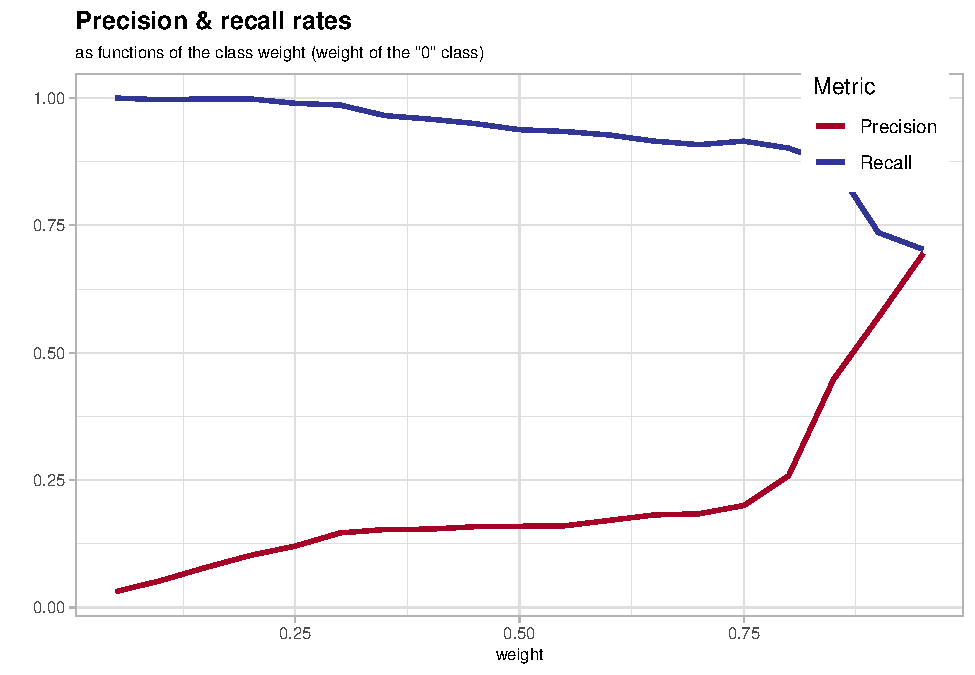
\includegraphics{credit_card_fraud_detection_files/figure-latex/finding_classwt1-1.pdf}

Our goal is to maximize recall, so after the analysis we decided to use
\(0.25\) for ``0'' class and \(0.75\) for ``1'' class, to balance our
data.

Now, we will fit a model with these parameters. We will use \(100\)
trees, because this setup gives us stable results.

\begin{Shaded}
\begin{Highlighting}[]
\NormalTok{forest }\OtherTok{\textless{}{-}} \FunctionTok{randomForest}\NormalTok{(}\FunctionTok{as\_factor}\NormalTok{(is\_fraud) }\SpecialCharTok{\textasciitilde{}}\NormalTok{ amt }\SpecialCharTok{+}\NormalTok{ age }\SpecialCharTok{+}\NormalTok{ category\_fraud }\SpecialCharTok{+}\NormalTok{ hour\_fraud,}
                       \AttributeTok{data=}\NormalTok{train\_cv, }
                       \AttributeTok{ntree=}\DecValTok{100}\NormalTok{, }
                       \AttributeTok{classwt =} \FunctionTok{c}\NormalTok{(}\StringTok{\textquotesingle{}0\textquotesingle{}} \OtherTok{=} \FloatTok{0.25}\NormalTok{, }\StringTok{\textquotesingle{}1\textquotesingle{}} \OtherTok{=} \FloatTok{0.75}\NormalTok{))}
\end{Highlighting}
\end{Shaded}

We will take a look at the confusion matrix:

\begin{Shaded}
\begin{Highlighting}[]
\NormalTok{conf\_mat\_forest\_train }\OtherTok{\textless{}{-}} \FunctionTok{confusion\_matrix}\NormalTok{(forest, train\_cv, }\StringTok{\textquotesingle{}is\_fraud\textquotesingle{}}\NormalTok{, }\AttributeTok{model\_type =} \StringTok{"forest"}\NormalTok{)}
\NormalTok{conf\_mat\_forest\_valid }\OtherTok{\textless{}{-}} \FunctionTok{confusion\_matrix}\NormalTok{(forest, valid\_cv, }\StringTok{\textquotesingle{}is\_fraud\textquotesingle{}}\NormalTok{, }\AttributeTok{model\_type =} \StringTok{"forest"}\NormalTok{)}
\NormalTok{conf\_mat\_forest\_train}
\end{Highlighting}
\end{Shaded}

\begin{verbatim}
## [1] 0.07620053 0.97157476
\end{verbatim}

\begin{Shaded}
\begin{Highlighting}[]
\NormalTok{conf\_mat\_forest\_valid}
\end{Highlighting}
\end{Shaded}

\begin{verbatim}
## [1] 0.07370642 0.95603410
\end{verbatim}

The model gives us very promising outcomes: on the training set recall
equals 0.972 and precision is 0.076, while on the testing set it is
0.956 and 0.074, accordingly.

\hypertarget{cross-validation-1}{%
\chapter{Cross validation}\label{cross-validation-1}}

For the cross validation we will use a function \texttt{crossv\_mc},
which conducts Monte Carlo Cross Validation. Also, we will not analyse
logistic regression with PCA, as this model gives not better results
than the basic logistic regression and lacks the possibility of
interpretation.

\hypertarget{logistic-regression-1}{%
\section{Logistic regression}\label{logistic-regression-1}}

First, we will take a look at the logistic regression. To do that, we
will sample a subset of our data, containing \(100000\) observations.

\begin{Shaded}
\begin{Highlighting}[]
\FunctionTok{set.seed}\NormalTok{(}\DecValTok{125}\NormalTok{)}
\NormalTok{n\_obs }\OtherTok{\textless{}{-}} \FloatTok{1e5}
\NormalTok{subset }\OtherTok{\textless{}{-}} \FunctionTok{sample\_n}\NormalTok{(}
\NormalTok{  data\_train\_bin[,}\FunctionTok{c}\NormalTok{(}\StringTok{"is\_fraud"}\NormalTok{, }\StringTok{"amt"}\NormalTok{, }\StringTok{"age"}\NormalTok{, }\StringTok{"category\_fraud"}\NormalTok{, }\StringTok{"hour\_fraud"}\NormalTok{)], }
\NormalTok{  n\_obs) }
\NormalTok{test\_ratio }\OtherTok{\textless{}{-}} \FloatTok{0.2}
\NormalTok{N }\OtherTok{\textless{}{-}} \DecValTok{200}

\CommentTok{\# Creating train/test sets}
\NormalTok{cv\_mc }\OtherTok{\textless{}{-}} \FunctionTok{crossv\_mc}\NormalTok{(subset, N, }\AttributeTok{test=}\NormalTok{test\_ratio)}

\CommentTok{\# fitting models on the training sets}
\NormalTok{models }\OtherTok{\textless{}{-}} \FunctionTok{map}\NormalTok{(cv\_mc}\SpecialCharTok{$}\NormalTok{train, }\SpecialCharTok{\textasciitilde{}} \FunctionTok{glm}\NormalTok{(is\_fraud }\SpecialCharTok{\textasciitilde{}}\NormalTok{ category\_fraud }\SpecialCharTok{+}\NormalTok{ amt }\SpecialCharTok{+}\NormalTok{ hour\_fraud }\SpecialCharTok{+}\NormalTok{ age}\SpecialCharTok{:}\NormalTok{hour\_fraud }\SpecialCharTok{+} 
\NormalTok{                                   amt}\SpecialCharTok{:}\NormalTok{hour\_fraud }\SpecialCharTok{+}\NormalTok{ amt}\SpecialCharTok{:}\NormalTok{category\_fraud }\SpecialCharTok{+}\NormalTok{ age}\SpecialCharTok{:}\NormalTok{category\_fraud,}
                                 \AttributeTok{data=}\NormalTok{., }\AttributeTok{family=}\NormalTok{binomial))}

\NormalTok{recalls\_train }\OtherTok{\textless{}{-}} \FunctionTok{map2\_dbl}\NormalTok{(models, cv\_mc}\SpecialCharTok{$}\NormalTok{train,}
                          \SpecialCharTok{\textasciitilde{}}\FunctionTok{confusion\_matrix}\NormalTok{(}\AttributeTok{model=}\NormalTok{.x, }\AttributeTok{data=}\FunctionTok{as\_tibble}\NormalTok{(.y), }\AttributeTok{col=}\StringTok{\textquotesingle{}is\_fraud\textquotesingle{}}\NormalTok{,}
                                            \AttributeTok{cutoff=}\FloatTok{0.003}\NormalTok{)[}\DecValTok{2}\NormalTok{])}

\NormalTok{precisions\_train }\OtherTok{\textless{}{-}} \FunctionTok{map2\_dbl}\NormalTok{(models, cv\_mc}\SpecialCharTok{$}\NormalTok{train,}
                             \SpecialCharTok{\textasciitilde{}}\FunctionTok{confusion\_matrix}\NormalTok{(}\AttributeTok{model=}\NormalTok{.x, }\AttributeTok{data=}\FunctionTok{as\_tibble}\NormalTok{(.y), }\AttributeTok{col=}\StringTok{\textquotesingle{}is\_fraud\textquotesingle{}}\NormalTok{,}
                                               \AttributeTok{cutoff=}\FloatTok{0.003}\NormalTok{)[}\DecValTok{1}\NormalTok{])}

\NormalTok{recalls\_test }\OtherTok{\textless{}{-}} \FunctionTok{map2\_dbl}\NormalTok{(models, cv\_mc}\SpecialCharTok{$}\NormalTok{test,}
                         \SpecialCharTok{\textasciitilde{}}\FunctionTok{confusion\_matrix}\NormalTok{(}\AttributeTok{model=}\NormalTok{.x, }\AttributeTok{data=}\FunctionTok{as\_tibble}\NormalTok{(.y), }\AttributeTok{col=}\StringTok{\textquotesingle{}is\_fraud\textquotesingle{}}\NormalTok{,}
                                           \AttributeTok{cutoff=}\FloatTok{0.003}\NormalTok{)[}\DecValTok{2}\NormalTok{])}

\NormalTok{precisions\_test }\OtherTok{\textless{}{-}} \FunctionTok{map2\_dbl}\NormalTok{(models, cv\_mc}\SpecialCharTok{$}\NormalTok{test,}
                            \SpecialCharTok{\textasciitilde{}}\FunctionTok{confusion\_matrix}\NormalTok{(}\AttributeTok{model=}\NormalTok{.x, }\AttributeTok{data=}\FunctionTok{as\_tibble}\NormalTok{(.y), }\AttributeTok{col=}\StringTok{\textquotesingle{}is\_fraud\textquotesingle{}}\NormalTok{,}
                                              \AttributeTok{cutoff=}\FloatTok{0.003}\NormalTok{)[}\DecValTok{1}\NormalTok{])}

\NormalTok{recalls\_all }\OtherTok{\textless{}{-}} \FunctionTok{rbind}\NormalTok{(}\FunctionTok{data.table}\NormalTok{(}\AttributeTok{model =} \StringTok{\textquotesingle{}train\_data\textquotesingle{}}\NormalTok{, }
                                \AttributeTok{recalls =}\NormalTok{ recalls\_train),}
                     \FunctionTok{data.table}\NormalTok{(}\AttributeTok{model =} \StringTok{\textquotesingle{}test\_data\textquotesingle{}}\NormalTok{, }
                                \AttributeTok{recalls =}\NormalTok{ recalls\_test))}

\NormalTok{precisions\_all }\OtherTok{\textless{}{-}} \FunctionTok{rbind}\NormalTok{(}\FunctionTok{data.table}\NormalTok{(}\AttributeTok{model =} \StringTok{\textquotesingle{}train\_data\textquotesingle{}}\NormalTok{, }
                                   \AttributeTok{precisions =}\NormalTok{ precisions\_train),}
                        \FunctionTok{data.table}\NormalTok{(}\AttributeTok{model =} \StringTok{\textquotesingle{}test\_data\textquotesingle{}}\NormalTok{, }
                                   \AttributeTok{precisions =}\NormalTok{ precisions\_test))}

\FunctionTok{cv\_metrics\_plt}\NormalTok{(recalls\_all, }\StringTok{"logistic regression"}\NormalTok{)}
\end{Highlighting}
\end{Shaded}

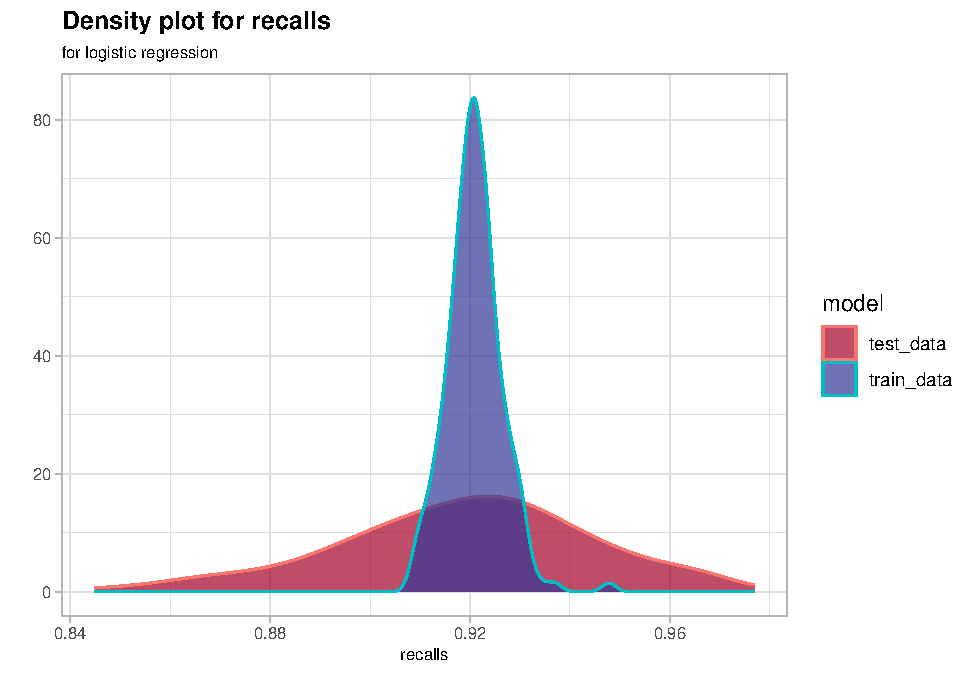
\includegraphics{credit_card_fraud_detection_files/figure-latex/cv_logreg-1.pdf}

\begin{Shaded}
\begin{Highlighting}[]
\FunctionTok{cv\_metrics\_plt}\NormalTok{(precisions\_all, }\StringTok{"logistics regression"}\NormalTok{)}
\end{Highlighting}
\end{Shaded}

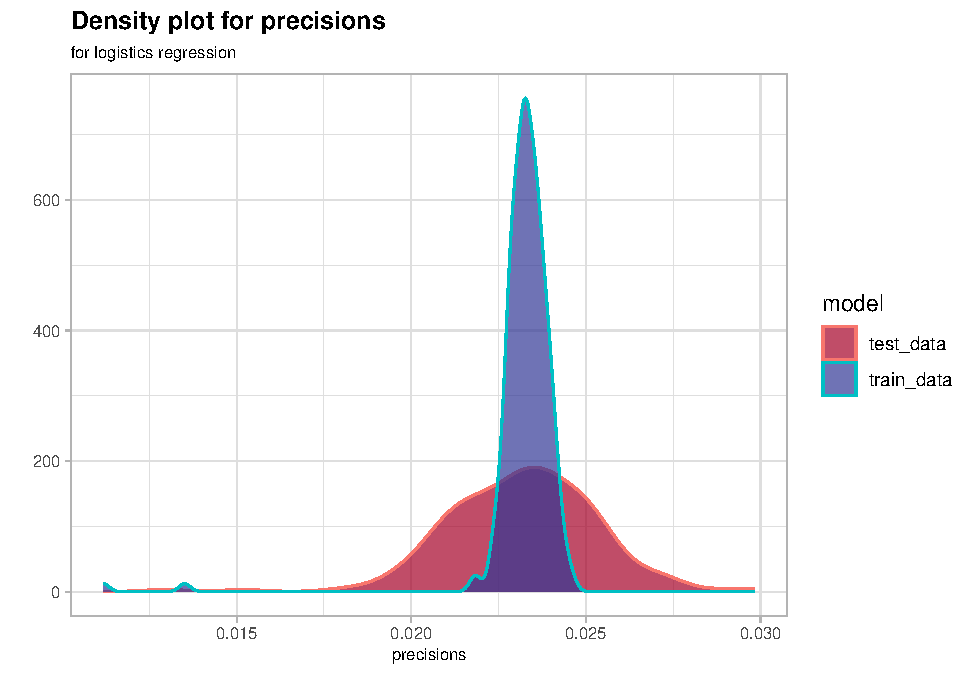
\includegraphics{credit_card_fraud_detection_files/figure-latex/cv_logreg-2.pdf}

We can see on the density plots, that recall is high, the density for
the testing set is wider, but no serious overfitting can be seen. The
precision is very low, but also the densities for the training and the
testing sets look similar.

\hypertarget{random-forest-1}{%
\section{Random forest}\label{random-forest-1}}

Now, we will do the same for the random forest.

\begin{Shaded}
\begin{Highlighting}[]
\FunctionTok{set.seed}\NormalTok{(}\DecValTok{125}\NormalTok{)}
\NormalTok{n\_obs }\OtherTok{\textless{}{-}} \FloatTok{1e5}
\NormalTok{subset }\OtherTok{\textless{}{-}} \FunctionTok{sample\_n}\NormalTok{(}
\NormalTok{  data\_train[,}\FunctionTok{c}\NormalTok{(}\StringTok{"is\_fraud"}\NormalTok{, }\StringTok{"amt"}\NormalTok{, }\StringTok{"age"}\NormalTok{, }\StringTok{"category\_fraud"}\NormalTok{, }\StringTok{"hour\_fraud"}\NormalTok{)], }
\NormalTok{  n\_obs) }
\NormalTok{test\_ratio }\OtherTok{\textless{}{-}} \FloatTok{0.2}
\NormalTok{N }\OtherTok{\textless{}{-}} \DecValTok{200}

\CommentTok{\# Creating train/test sets}
\NormalTok{cv\_mc }\OtherTok{\textless{}{-}} \FunctionTok{crossv\_mc}\NormalTok{(subset, N, }\AttributeTok{test=}\NormalTok{test\_ratio)}

\CommentTok{\# fitting models on the training sets}
\NormalTok{models }\OtherTok{\textless{}{-}} \FunctionTok{map}\NormalTok{(cv\_mc}\SpecialCharTok{$}\NormalTok{train, }\SpecialCharTok{\textasciitilde{}} \FunctionTok{randomForest}\NormalTok{(}\FunctionTok{as\_factor}\NormalTok{(is\_fraud) }\SpecialCharTok{\textasciitilde{}}\NormalTok{ amt }\SpecialCharTok{+}\NormalTok{ age }\SpecialCharTok{+}\NormalTok{ category\_fraud }\SpecialCharTok{+}\NormalTok{ hour\_fraud,}
                                          \AttributeTok{data=}\NormalTok{., }\AttributeTok{ntree=}\DecValTok{100}\NormalTok{, }\AttributeTok{classwt =} \FunctionTok{c}\NormalTok{(}\StringTok{\textquotesingle{}0\textquotesingle{}} \OtherTok{=} \FloatTok{0.25}\NormalTok{, }\StringTok{\textquotesingle{}1\textquotesingle{}} \OtherTok{=} \FloatTok{0.75}\NormalTok{)))}

\NormalTok{recalls\_train }\OtherTok{\textless{}{-}} \FunctionTok{map2\_dbl}\NormalTok{(models, cv\_mc}\SpecialCharTok{$}\NormalTok{train,}
                          \SpecialCharTok{\textasciitilde{}}\FunctionTok{confusion\_matrix}\NormalTok{(}\AttributeTok{model=}\NormalTok{.x, }\AttributeTok{data=}\FunctionTok{as\_tibble}\NormalTok{(.y), }
                                            \AttributeTok{col=}\StringTok{\textquotesingle{}is\_fraud\textquotesingle{}}\NormalTok{, }\AttributeTok{model\_type =} \StringTok{"forest"}\NormalTok{)[}\DecValTok{2}\NormalTok{])}

\NormalTok{precisions\_train }\OtherTok{\textless{}{-}} \FunctionTok{map2\_dbl}\NormalTok{(models, cv\_mc}\SpecialCharTok{$}\NormalTok{train,}
                             \SpecialCharTok{\textasciitilde{}}\FunctionTok{confusion\_matrix}\NormalTok{(}\AttributeTok{model=}\NormalTok{.x, }\AttributeTok{data=}\FunctionTok{as\_tibble}\NormalTok{(.y), }
                                               \AttributeTok{col=}\StringTok{\textquotesingle{}is\_fraud\textquotesingle{}}\NormalTok{, }\AttributeTok{model\_type =} \StringTok{"forest"}\NormalTok{)[}\DecValTok{1}\NormalTok{])}

\NormalTok{recalls\_test }\OtherTok{\textless{}{-}} \FunctionTok{map2\_dbl}\NormalTok{(models, cv\_mc}\SpecialCharTok{$}\NormalTok{test,}
                         \SpecialCharTok{\textasciitilde{}}\FunctionTok{confusion\_matrix}\NormalTok{(}\AttributeTok{model=}\NormalTok{.x, }\AttributeTok{data=}\FunctionTok{as\_tibble}\NormalTok{(.y), }
                                           \AttributeTok{col=}\StringTok{\textquotesingle{}is\_fraud\textquotesingle{}}\NormalTok{, }\AttributeTok{model\_type =} \StringTok{"forest"}\NormalTok{)[}\DecValTok{2}\NormalTok{])}

\NormalTok{precisions\_test }\OtherTok{\textless{}{-}} \FunctionTok{map2\_dbl}\NormalTok{(models, cv\_mc}\SpecialCharTok{$}\NormalTok{test,}
                            \SpecialCharTok{\textasciitilde{}}\FunctionTok{confusion\_matrix}\NormalTok{(}\AttributeTok{model=}\NormalTok{.x, }\AttributeTok{data=}\FunctionTok{as\_tibble}\NormalTok{(.y), }
                                              \AttributeTok{col=}\StringTok{\textquotesingle{}is\_fraud\textquotesingle{}}\NormalTok{, }\AttributeTok{model\_type =} \StringTok{"forest"}\NormalTok{)[}\DecValTok{1}\NormalTok{])}

\NormalTok{recalls\_all }\OtherTok{\textless{}{-}} \FunctionTok{rbind}\NormalTok{(}\FunctionTok{tibble}\NormalTok{(}\AttributeTok{model =} \StringTok{\textquotesingle{}train\_data\textquotesingle{}}\NormalTok{, }\AttributeTok{recalls =}\NormalTok{ recalls\_train),}
                     \FunctionTok{tibble}\NormalTok{(}\AttributeTok{model =} \StringTok{\textquotesingle{}test\_data\textquotesingle{}}\NormalTok{, }\AttributeTok{recalls =}\NormalTok{ recalls\_test))}

\NormalTok{precisions\_all }\OtherTok{\textless{}{-}} \FunctionTok{rbind}\NormalTok{(}\FunctionTok{tibble}\NormalTok{(}\AttributeTok{model =} \StringTok{\textquotesingle{}train\_data\textquotesingle{}}\NormalTok{, }\AttributeTok{precisions =}\NormalTok{ precisions\_train),}
                        \FunctionTok{tibble}\NormalTok{(}\AttributeTok{model =} \StringTok{\textquotesingle{}test\_data\textquotesingle{}}\NormalTok{, }\AttributeTok{precisions =}\NormalTok{ precisions\_test))}

\CommentTok{\# Density plot of metrics}
\FunctionTok{cv\_metrics\_plt}\NormalTok{(recalls\_all, }\StringTok{"random forest"}\NormalTok{)}
\end{Highlighting}
\end{Shaded}

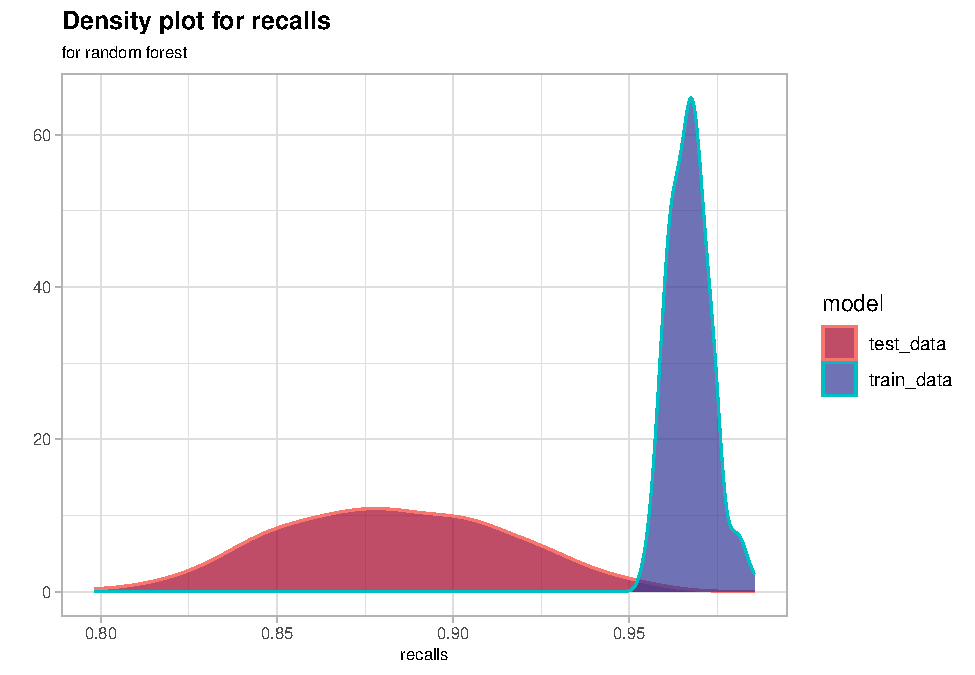
\includegraphics{credit_card_fraud_detection_files/figure-latex/cv_rf-1.pdf}

\begin{Shaded}
\begin{Highlighting}[]
\FunctionTok{cv\_metrics\_plt}\NormalTok{(precisions\_all, }\StringTok{"random forest"}\NormalTok{)}
\end{Highlighting}
\end{Shaded}

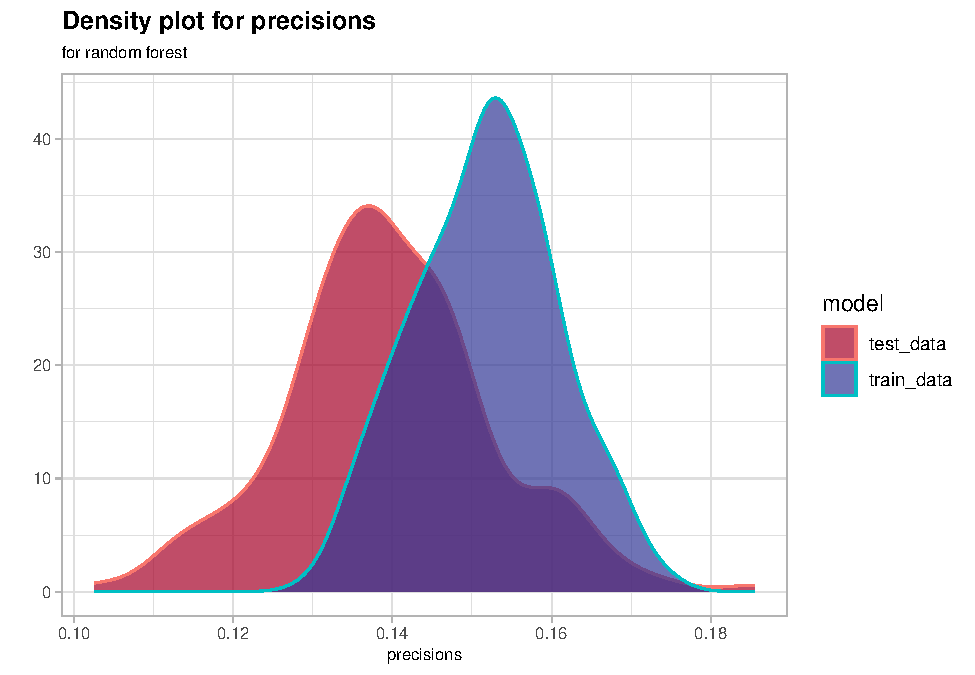
\includegraphics{credit_card_fraud_detection_files/figure-latex/cv_rf-2.pdf}

Here, we can see that the model overfits quite seriously, although the
metrics for the testing set are still relatively high. The overfit can
be seen on the recall, which is not surprising, because we were focusing
on finding the parameters that maximize this metric, so the model is not
as robust as it should be.

\hypertarget{conclusion}{%
\chapter{Conclusion}\label{conclusion}}

Comparing the three models, the logistic regression gives the best
recall and also do not overfit much. On the other hand, even though the
random forest overfits our data heavily, it gives not much lower recall
on the testing set and also much higher precision. The PCA for the
logistic regression model gives similar results as the basic logistic
regression, while it does not provide possibility to interpret the
model. For that reasons, we reject this model for our problem.

\begin{longtable}[]{@{}
  >{\raggedright\arraybackslash}p{(\columnwidth - 10\tabcolsep) * \real{0.2000}}
  >{\raggedright\arraybackslash}p{(\columnwidth - 10\tabcolsep) * \real{0.2400}}
  >{\raggedleft\arraybackslash}p{(\columnwidth - 10\tabcolsep) * \real{0.1300}}
  >{\raggedleft\arraybackslash}p{(\columnwidth - 10\tabcolsep) * \real{0.1600}}
  >{\raggedleft\arraybackslash}p{(\columnwidth - 10\tabcolsep) * \real{0.1200}}
  >{\raggedleft\arraybackslash}p{(\columnwidth - 10\tabcolsep) * \real{0.1500}}@{}}
\caption{Table with results for the logistic regression and the random
forest.}\tabularnewline
\toprule()
\begin{minipage}[b]{\linewidth}\raggedright
Model
\end{minipage} & \begin{minipage}[b]{\linewidth}\raggedright
Quality
\end{minipage} & \begin{minipage}[b]{\linewidth}\raggedleft
Recall\_train
\end{minipage} & \begin{minipage}[b]{\linewidth}\raggedleft
Precision\_train
\end{minipage} & \begin{minipage}[b]{\linewidth}\raggedleft
Recall\_test
\end{minipage} & \begin{minipage}[b]{\linewidth}\raggedleft
Precision\_test
\end{minipage} \\
\midrule()
\endfirsthead
\toprule()
\begin{minipage}[b]{\linewidth}\raggedright
Model
\end{minipage} & \begin{minipage}[b]{\linewidth}\raggedright
Quality
\end{minipage} & \begin{minipage}[b]{\linewidth}\raggedleft
Recall\_train
\end{minipage} & \begin{minipage}[b]{\linewidth}\raggedleft
Precision\_train
\end{minipage} & \begin{minipage}[b]{\linewidth}\raggedleft
Recall\_test
\end{minipage} & \begin{minipage}[b]{\linewidth}\raggedleft
Precision\_test
\end{minipage} \\
\midrule()
\endhead
logistic regression & not overfited & 0.928 & 0.022 & 0.902 & 0.015 \\
random forest & significantly overfited & 0.972 & 0.076 & 0.911 &
0.015 \\
\bottomrule()
\end{longtable}

We think that the logistic regression is more transparent and in this
case also more robust, while the random forest is better in terms of not
giving too many false alarms. We would recommend implementing the model
\texttt{logreg} for now. On the other hand, we believe, that random
forest could give better results in the long run, if implemented with
additional variables like ``time from the last transaction'' or ``number
of transactions made on the same day''.

Overall, for now we recommend the model \texttt{logreg} as the best of
the models presented in this paper.

\end{document}
